%\documentclass[a4,semhelv,landscape]{seminar}
\documentclass[landscape]{slides}
%\documentclass[pdf, default, slideBW, nocolorBG]{prosper}
\usepackage[left=0.2cm,top=0.2cm,right=0.2cm,bottom=0.2cm,nohead,nofoot]{geometry}
%\def\everyslide{\sffamily}
%\usepackage{fullpage}
\usepackage{graphicx}
\usepackage[usenames]{color}
%\usepackage{color}
\usepackage{verbatim}
\usepackage{nopageno}
\usepackage{setspace}
%\usepackage{times}
% define some nice colors
\definecolor{myred}{rgb}{0.6,0,0}
\definecolor{myblue}{rgb}{0,0.2,0.4}
\definecolor{mygreen}{rgb}{0,0.5,0.0}
\definecolor{mypurple}{cmyk}{0.5,1.0,0.0,0.0}
\definecolor{myorange}{cmyk}{0.0,0.75,1.0,0.0}
%\color{myblue}

\begin{document}
%%%%%%%%%%%%%%%%%%%%%%%%%%%%%%%%%%%%%%%%%%%%%%%%%%%%%%%%%%%%%%%%%%%%
%Slide 0 - title
\begin{slide}
\begin{center}
\large{\textbf{Reference-based viral sequence annotation using VADR}}

\normalsize

Eric Nawrocki \\

\medskip

\medskip

\medskip

\medskip

\medskip

\small
\begin{tabular}{c}
%Alejandro Sch\"{a}ffer's group \\
%\\
National Center for Biotechnology Information\\
National Institutes of Health\\
\\
\end{tabular}

\vspace{0.1in}


\includegraphics[width=2.5in]{figs/ncbi-logo}

\end{center}
\end{slide}
%%%%%%%%%%%%%%%%%%%%%%%%%%%%%%%%%%%%%%%%%%%%%%%%%%%%%%%%%%%%%%%%%%%%%%
\begin{slide}
\begin{center}
\textbf{GenBank has a lot of sequence data}
\end{center}


\includegraphics[width=9in]{figs/genbank-2019-title}

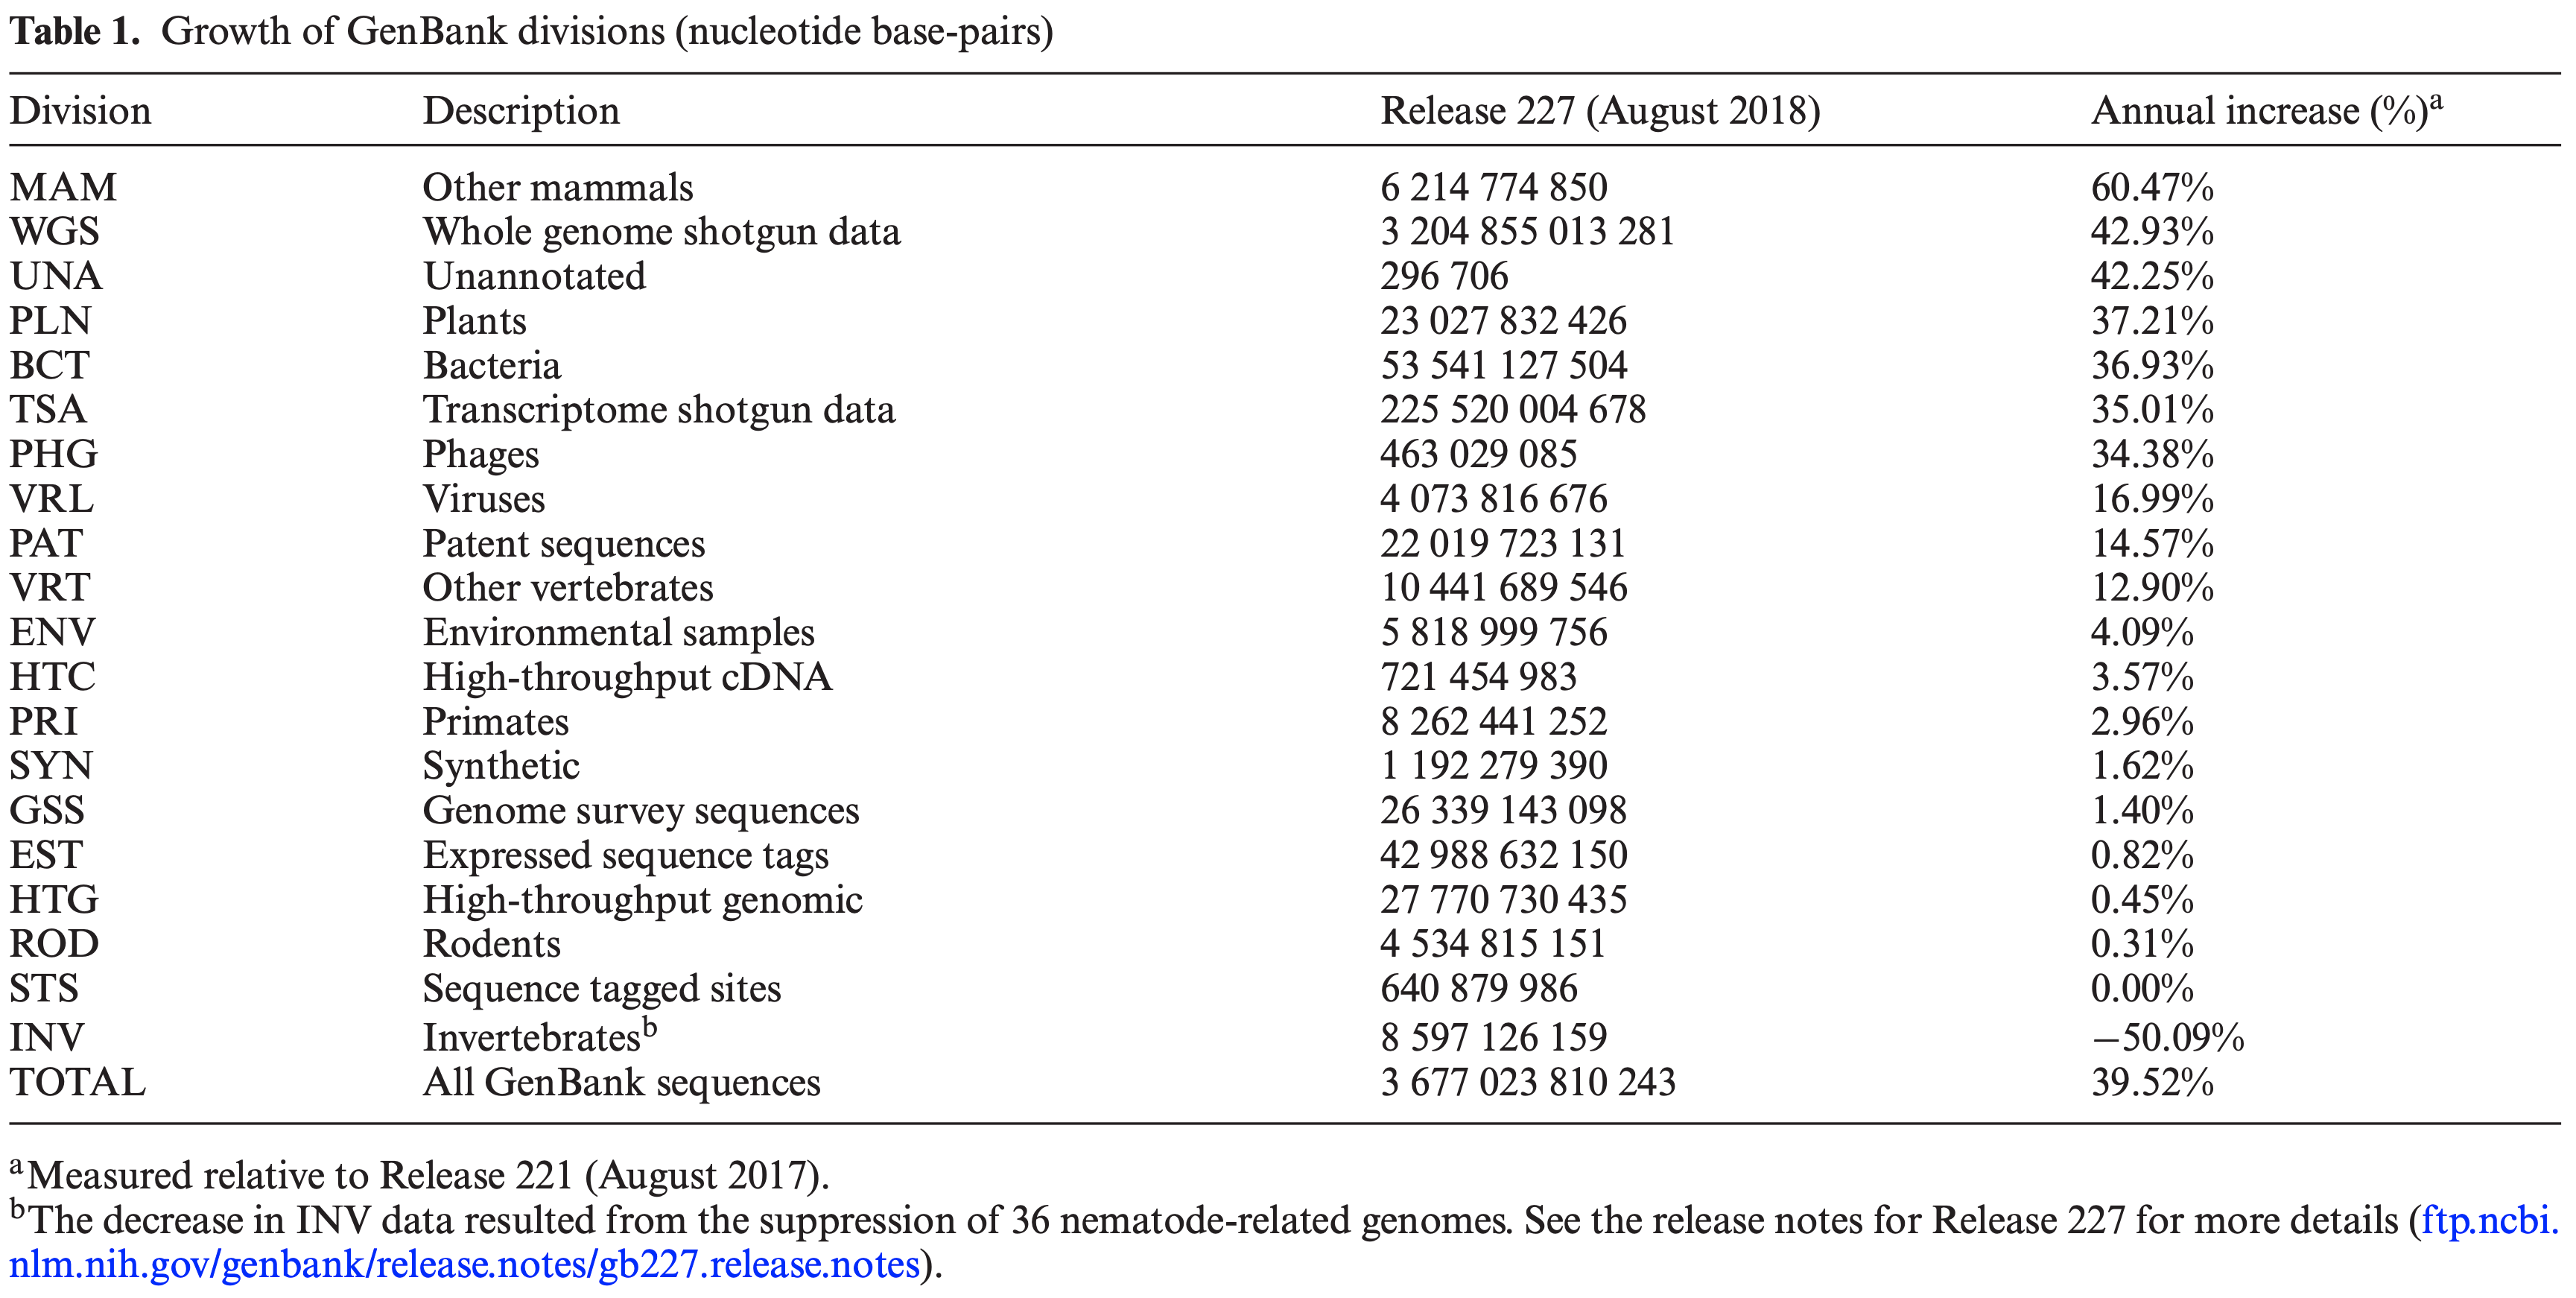
\includegraphics[width=9in]{figs/genbank-2019-table1}


\vfill
\end{slide}
%%%%%%%%%%%%%%%%%%%%%%%%%%%%%%%%%%%%%%%%%%%%%%%%%%%%%%%%%%%%%%%%%%%%%%
\begin{slide}
\begin{center}
\textbf{Sequence submissions are handled by expert NCBI indexers}
\end{center}

\small
\begin{itemize}
\item Indexers check submissions for quality
\item Many submissions are of \emph{marker genes}, used to
  characterize environments (microbiome, soil), which are
  automatically analyzed by BLAST or specialized tools.
%\item Submissions with zero errors automatically enter database
%  (``foosh'')
%\item Submissions with errors can be corrected by submitter or are manually reviewed by an indexer
\end{itemize}

\medskip

\begin{center}
\begin{tabular}{lrr}
                                 &    2018  & total     \\
 marker gene/                    &  GenBank & GenBank   \\
 sequence type                   &  \# seqs & \# seqs   \\ \hline
& & \\
%\textcolor{red}{16S rRNA}        & \textcolor{red}{333,121}  & \textcolor{red}{8,015,297} & \textcolor{red}{18,262,402} & \textcolor{red}{BLAST}\footnote{TLS submissions now processed with Ribosensor} \\
%16S rRNA                        & 333,121  & 8,015,297 & 18,262,402 & BLAST$^{*}$ \\
16S rRNA                        & 333,121  & 8,015,297 \\
& & \\                    
 23S rRNA                        & 74,287  &   275,014  \\
& & \\
 ITS1                            & 27,279  &   359,380  \\
& & \\                    
 ITS2                            & 24,144  &   184,515  \\
& & \\                    
 ITS1+ITS2                       & 26,734  &   445,721  \\
& & \\                    
 COX1                            &      ?  &         ?  \\
& & \\                    
 Influenza                       & 74,868  &   665,464  \\
\end{tabular}
\end{center}
\vfill
%\tiny \flushleft{$\dagger$ TLS: Targeted Locus Study, currently only 16S submissions with $>=$ 2500 seqs, handled by Anji Johnston}
%\tiny \flushleft{$\ddagger$ TLS submissions now processed with ribosensor}
\end{slide}
%%%%%%%%%%%%%%%%%%%%%%%%%%%%%%%%%%%%%%%%%%%%%%%%%%%%%%%%%%%%%%%%%%%%%%
\begin{slide}
\begin{center}
\textbf{Manual NCBI GenBank indexing does not scale}

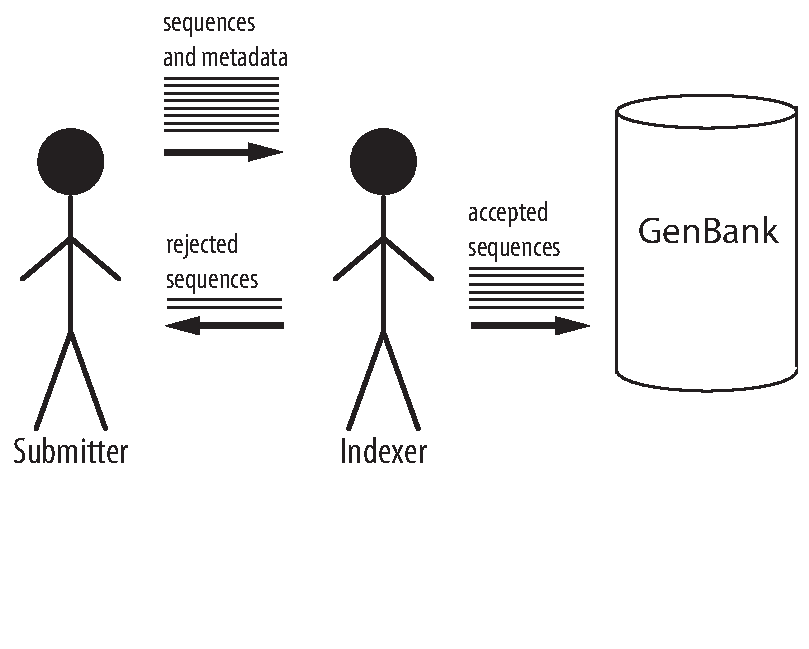
\includegraphics[width=7in]{figs/submission-schematic-1}

\vfill
\end{center}
\end{slide}
%%%%%%%%%%%%%%%%%%%%%%%%%%%%%%%%%%%%%%%%%%%%%%%%%%%%%%%%%%%%%%%%%%%%%%
\begin{slide}
\begin{center}
\textbf{NCBI GenBank Indexers use BLAST}

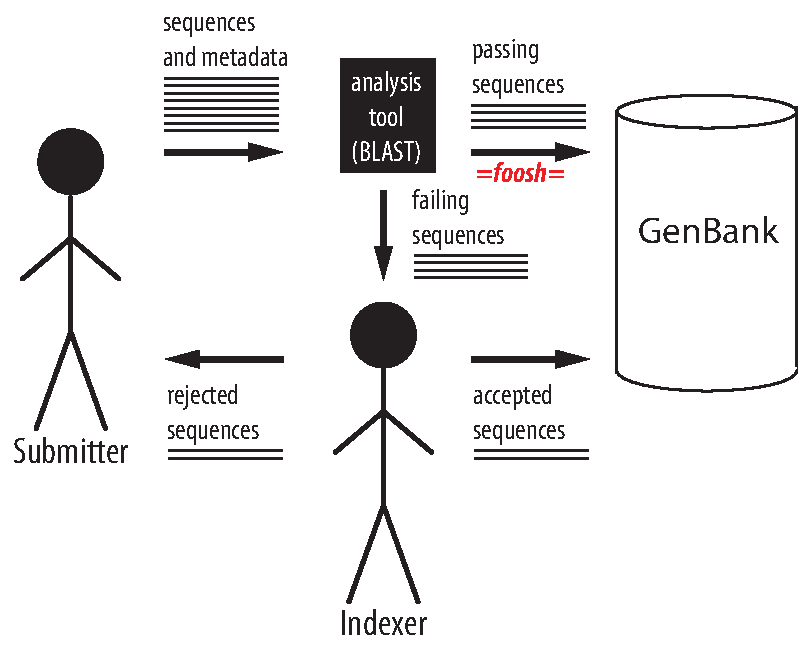
\includegraphics[width=7in]{figs/submission-schematic-2}

\small
\begin{itemize}
\item Foosh pipelines exist for 16S, 23S, ITS (BLAST-based) and
    Influenza (FLAN)
\end{itemize}

\vfill
\end{center}
\end{slide}
%%%%%%%%%%%%%%%%%%%%%%%%%%%%%%%%%%%%%%%%%%%%%%%%%%%%%%%%%%%%%%%%%%%%%%
\begin{slide}
\begin{center}
\textbf{NCBI GenBank Indexers use BLAST}

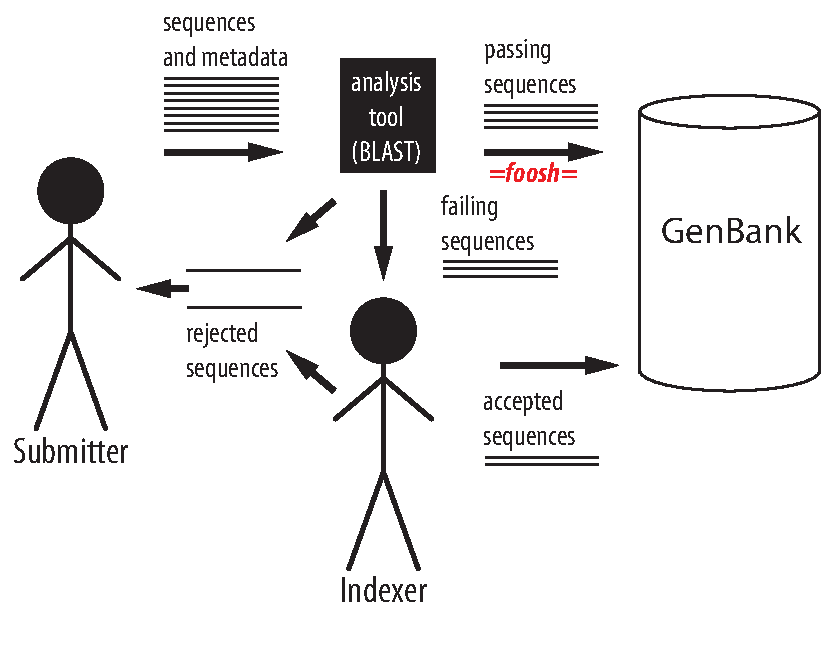
\includegraphics[width=7in]{figs/submission-schematic-3}

\small
\begin{itemize}
\item Foosh pipelines exist for 16S, 23S, ITS (BLAST-based) and
    Influenza (FLAN)
\end{itemize}

\vfill
\end{center}
\end{slide}
%%%%%%%%%%%%%%%%%%%%%%%%%%%%%%%%%%%%%%%%%%%%%%%%%%%%%%%%%%%%%%%%%%%%%%
\begin{slide}
\begin{center}

\textbf{Viruses with highest number of sequences in GenBank\footnote{as of October, 2019.}}

\tiny
\begin{tabular}{lrl}
species                   &       \#seqs & family           \\ \hline
%                                                              % taxids
& & \\
HIV-1                     &      850,115 & \emph{Retroviridae}     \\ % 11676
& & \\
Influenza A virus         &      684,026 & \emph{Orthomyxoviridae} \\ % 11320
& & \\
Hepacivirus C             &      244,533 & \emph{Flaviviridae}     \\ % 11103
& & \\
Hepatitis B virus         &      114,306 & \emph{Hepadnaviridae}   \\ % 10407
& & \\
Influenza B virus         &      100,373 & \emph{Orthomyxoviridae} \\ % 11520
& & \\
Rotavirus A               &       73,375 & \emph{Reoviridae}       \\ % 28875
& & \\
SIV                       &       44,374 & \emph{Retroviridae}     \\ % 11723
& & \\
Norovirus (Norwalk virus) &       40,925 & \emph{Caliciviridae}    \\ % 11983
& & \\
Enterovirus A             &       31,478 & \emph{Picornaviridae}   \\ % 138948
& & \\
PRRSV                     &       29,081 & \emph{Arteriviridae}    \\ % 28344
& & \\
Dengue virus              &       28,564 & \emph{Flaviviridae}     \\ % 12637
& & \\
Human orthopneumovirus    &       24,384 & \emph{Pneumoviridae}    \\ % 11250 (RSV) 
& & \\
Enterovirus B             &       23,865 & \emph{Picornaviridae}   \\ % 138949
& & \\
Rabies lyssavirus         &       23,771 & \emph{Rhabdoviridae}    \\ % 11292
& & \\
West Nile virus           &       21,563 & \emph{Flaviviridae}     \\ % 11082
& & \\
Measles morbillivirus     &       17,233 & \emph{Paramyxoviridae}  \\ % 11234
\end{tabular}

\vfill

\end{center}
\end{slide}

%%%%%%%%%%%%%%%%%%%%%%%%%%%%%%%%%%%%%%%%%%%%%%%%%%%%%%%%%%%%%%%%%%%%%%
\begin{slide}
\begin{center}
\textbf{Viral sequences are not systematically or thoroughly annotated}
\end{center}

\small
\begin{itemize}
\item Examples of incomplete annotation: 
  \begin{itemize}
  \item Rfam families are rarely to never annotated in viral genomes
    (roughly 200 families)
  \item Less than 2\% of Norovirus sequences have mature peptide
    annotation. 
\end{itemize}
\item Systematic and complete annotation would benefit viral
  researchers and facilitate \\ comparative analyses
\end{itemize}

\vfill
\end{slide}
%%%%%%%%%%%%%%%%%%%%%%%%%%%%%%%%%%%%%%%%%%%%%%%%%%%%%%%%%%%%%%%%%%%%%%
\begin{slide}
\begin{center}
\textbf{Viral sequences are not systematically or thoroughly annotated}
\end{center}

\small
\begin{itemize}
\item Examples of incomplete annotation: 
  \begin{itemize}
  \item Rfam families are rarely to never annotated in viral genomes
    (roughly 200 families)
  \item Less than 2\% of Norovirus sequences have mature peptide
    annotation. 
\end{itemize}
\item Systematic and complete annotation would benefit viral
  researchers and facilitate \\ comparative analyses
\end{itemize}

\begin{center}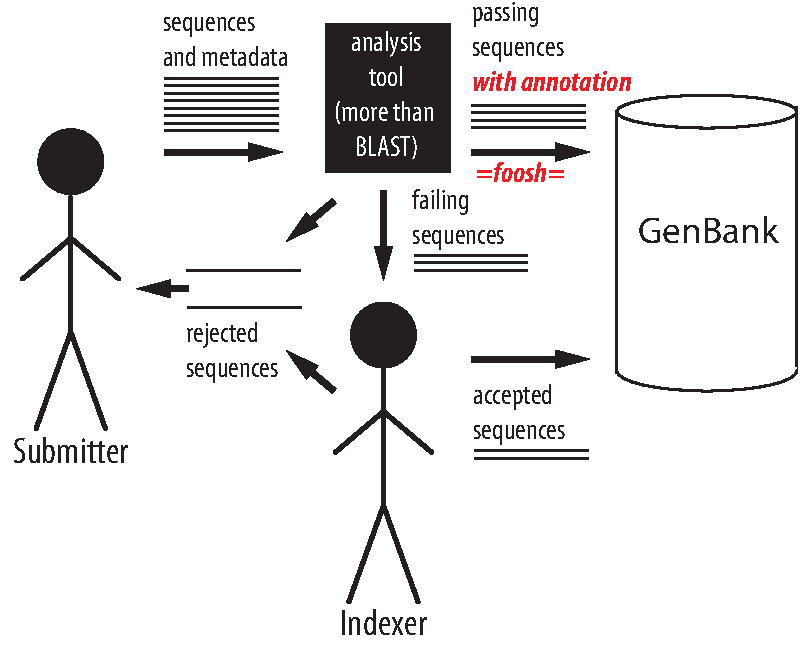
\includegraphics[width=7in]{figs/submission-schematic-4}\end{center}

\vfill
\end{slide}
%%%%%%%%%%%%%%%%%%%%%%%%%%%%%%%%%%%%%%%%%%%%%%%%%%%%%%%%%%%%%%%%%%%%%%
\begin{slide}
\begin{center}
VADR (Viral Annotation DefineR) \\ uses RefSeqs to validate and
annotate viral sequences

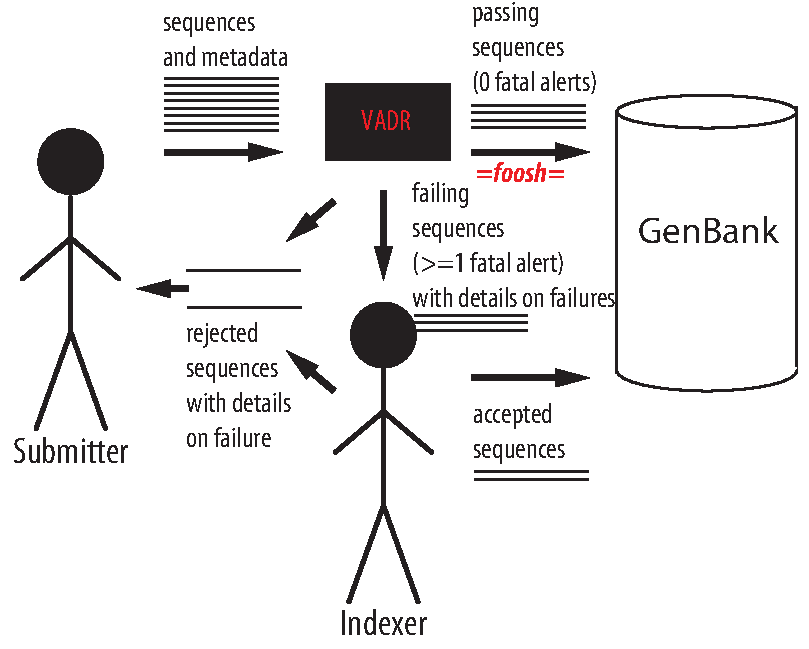
\includegraphics[width=7in]{figs/submission-schematic-5}
\end{center}

\small
\begin{itemize}
  \item Unexpected characteristics are reported as \emph{alerts}
    (e.g. early stop codon)
  \item Some alerts are \emph{fatal} and cause sequences to \emph{fail}.
\end{itemize}

%\small
%\begin{itemize}
%\item Build a model (covariance model) from a RefSeq (or alignment) using \texttt{v-build.pl}
%\begin{itemize}
%  \item includes boundaries of CDS, mat\_peptide, ncRNA and other features
%\end{itemize}

%\item Incoming sequences are compared against a library of models to find
%  the best-matching model which is used to annotate the sequence using
%  \texttt{v-annotate.pl}.

\vfill
\end{slide}
%%%%%%%%%%%%%%%%%%%%%%%%%%%%%%%%%%%%%%%%%%%%%%%%%%%%%%%%%%%%%%%%%%%%%%
\begin{slide}
\begin{center}

\textbf{Norovirus and Dengue virus chosen as first viruses for VADR testing}

\tiny
\begin{tabular}{lrl}
species                   &       \#seqs & family           \\ \hline
%                                                              % taxids
& & \\
HIV-1                     &      850,115 & \emph{Retroviridae}     \\ % 11676
& & \\
Influenza A virus         &      684,026 & \emph{Orthomyxoviridae} \\ % 11320
& & \\
Hepacivirus C             &      244,533 & \emph{Flaviviridae}     \\ % 11103
& & \\
Hepatitis B virus         &      114,306 & \emph{Hepadnaviridae}   \\ % 10407
& & \\
Influenza B virus         &      100,373 & \emph{Orthomyxoviridae} \\ % 11520
& & \\
Rotavirus A               &       73,375 & \emph{Reoviridae}       \\ % 28875
& & \\
SIV                       &       44,374 & \emph{Retroviridae}     \\ % 11723
& & \\
\textcolor{red}{Norovirus (Norwalk virus)} &       \textcolor{red}{40,925} & \textcolor{red}{\emph{Caliciviridae}}    \\ % 11983
& & \\
Enterovirus A             &       31,478 & \emph{Picornaviridae}   \\ % 138948
& & \\
PRRSV                     &       29,081 & \emph{Arteriviridae}    \\ % 28344
& & \\
%Dengue virus              &       28,564 & \emph{Flaviviridae}     \\ % 12637
\textcolor{red}{Dengue virus}              &       \textcolor{red}{28,564} & \textcolor{red}{\emph{Flaviviridae}}     \\ % 12637
& & \\
Human orthopneumovirus    &       24,384 & \emph{Pneumoviridae}    \\ % 11250 (RSV) 
& & \\
Enterovirus B             &       23,865 & \emph{Picornaviridae}   \\ % 138949
& & \\
Rabies lyssavirus         &       23,771 & \emph{Rhabdoviridae}    \\ % 11292
& & \\
West Nile virus           &       21,563 & \emph{Flaviviridae}     \\ % 11082
& & \\
Measles morbillivirus     &       17,233 & \emph{Paramyxoviridae}  \\ % 11234
\end{tabular}

\vfill

\end{center}
\end{slide}

%%%%%%%%%%%%%%%%%%%%%%%%%%%%%%%%%%%%%%%%%%%%%%%%%%%%%%%%%%%%%%%%%%%%%%
\begin{slide}
\begin{center}
\textbf{VADR build step (\texttt{v-build.pl}) builds a homology model
  \\ (covariance model (CM)) of a RefSeq and stores feature information}

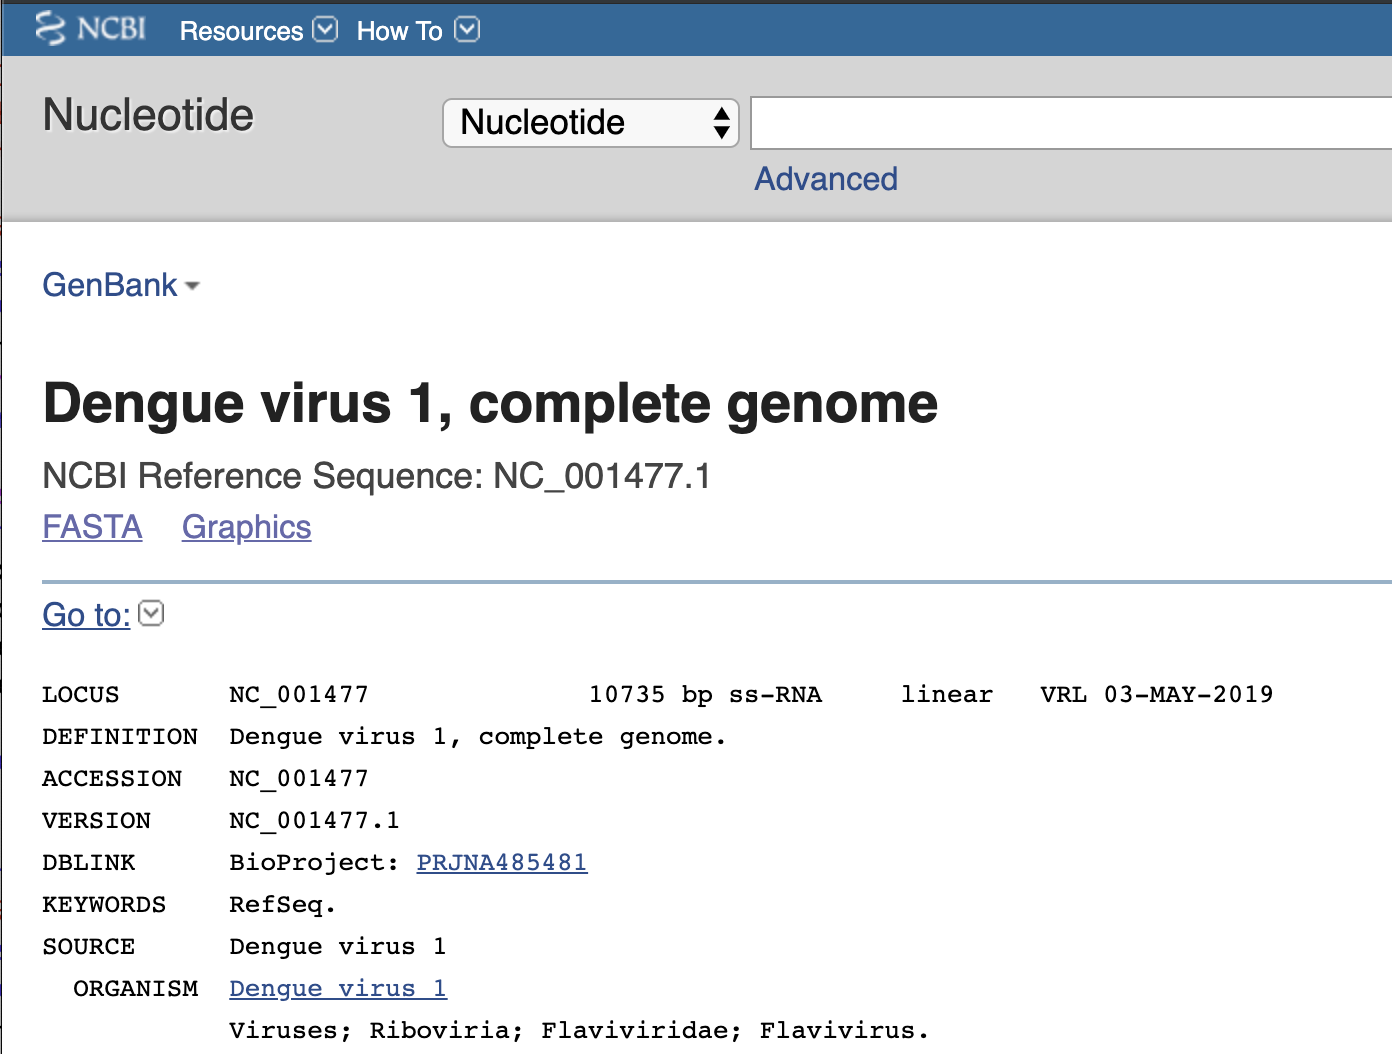
\includegraphics[width=6in]{figs/ss-001477-top}

\end{center}
\vfill
\end{slide}
%%%%%%%%%%%%%%%%%%%%%%%%%%%%%%%%%%%%%%%%%%%%%%%%%%%%%%%%%%%%%%%%%%%%%%
\begin{slide}
\begin{center}
\textbf{VADR build step (\texttt{v-build.pl}) builds a homology model
  \\ (covariance model (CM)) of a RefSeq and stores feature information}

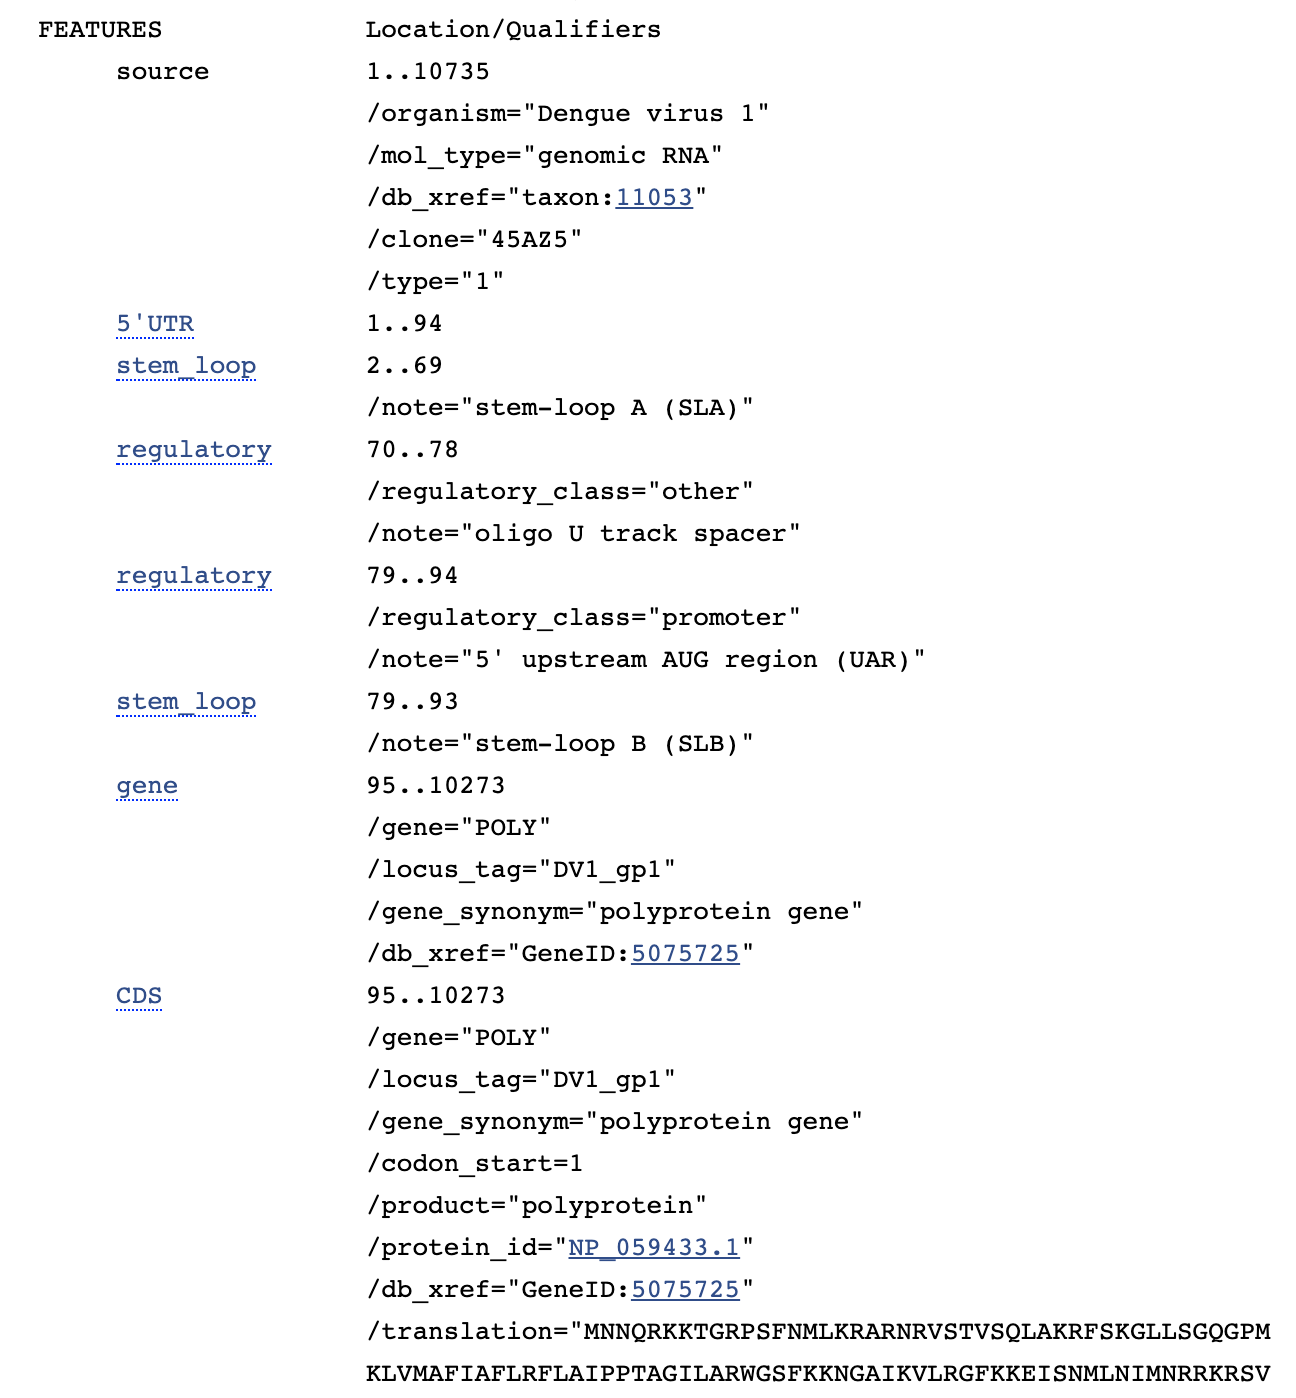
\includegraphics[width=6in]{figs/ss-001477-mid}

\end{center}
\vfill
\end{slide}
%%%%%%%%%%%%%%%%%%%%%%%%%%%%%%%%%%%%%%%%%%%%%%%%%%%%%%%%%%%%%%%%%%%%%%
\begin{slide}
\begin{center}
\textbf{VADR build step (\texttt{v-build.pl}) builds a homology model
  \\ (covariance model (CM)) of a RefSeq and stores feature information}

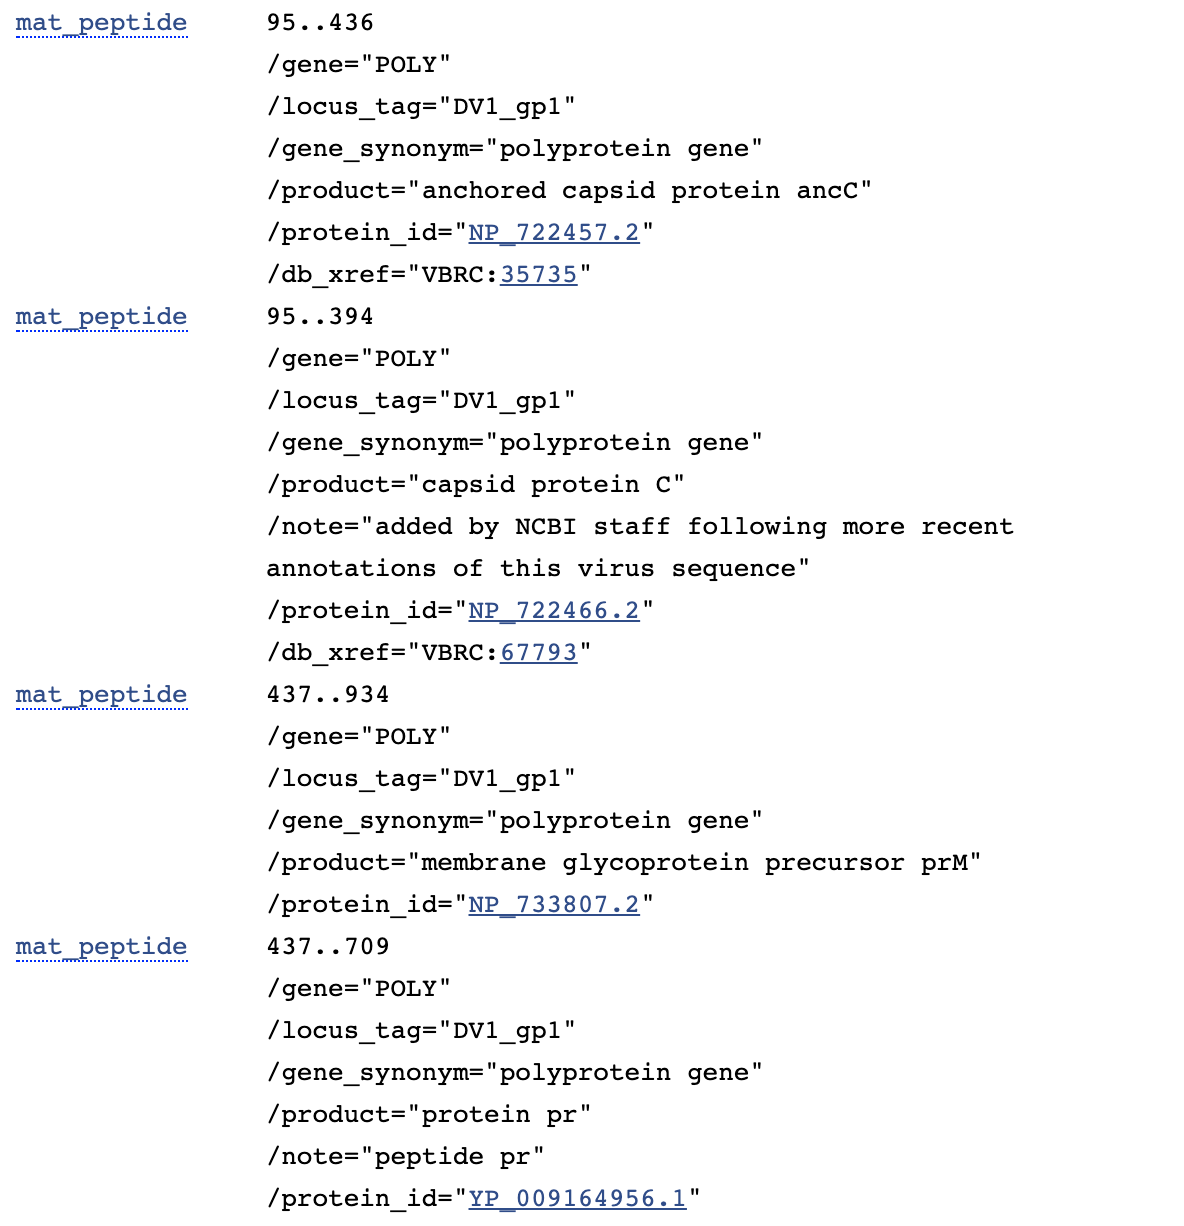
\includegraphics[width=6in]{figs/ss-001477-bot}

\end{center}
\vfill
\end{slide}
%%%%%%%%%%%%%%%%%%%%%%%%%%%%%%%%%%%%%%%%%%%%%%%%%%%%%%%%%%%%%%%%%%%%%%
\begin{slide}
\begin{center}
\textbf{VADR build step (\texttt{v-build.pl}) builds a homology model
  \\ (covariance model (CM)) of a RefSeq and stores feature information}

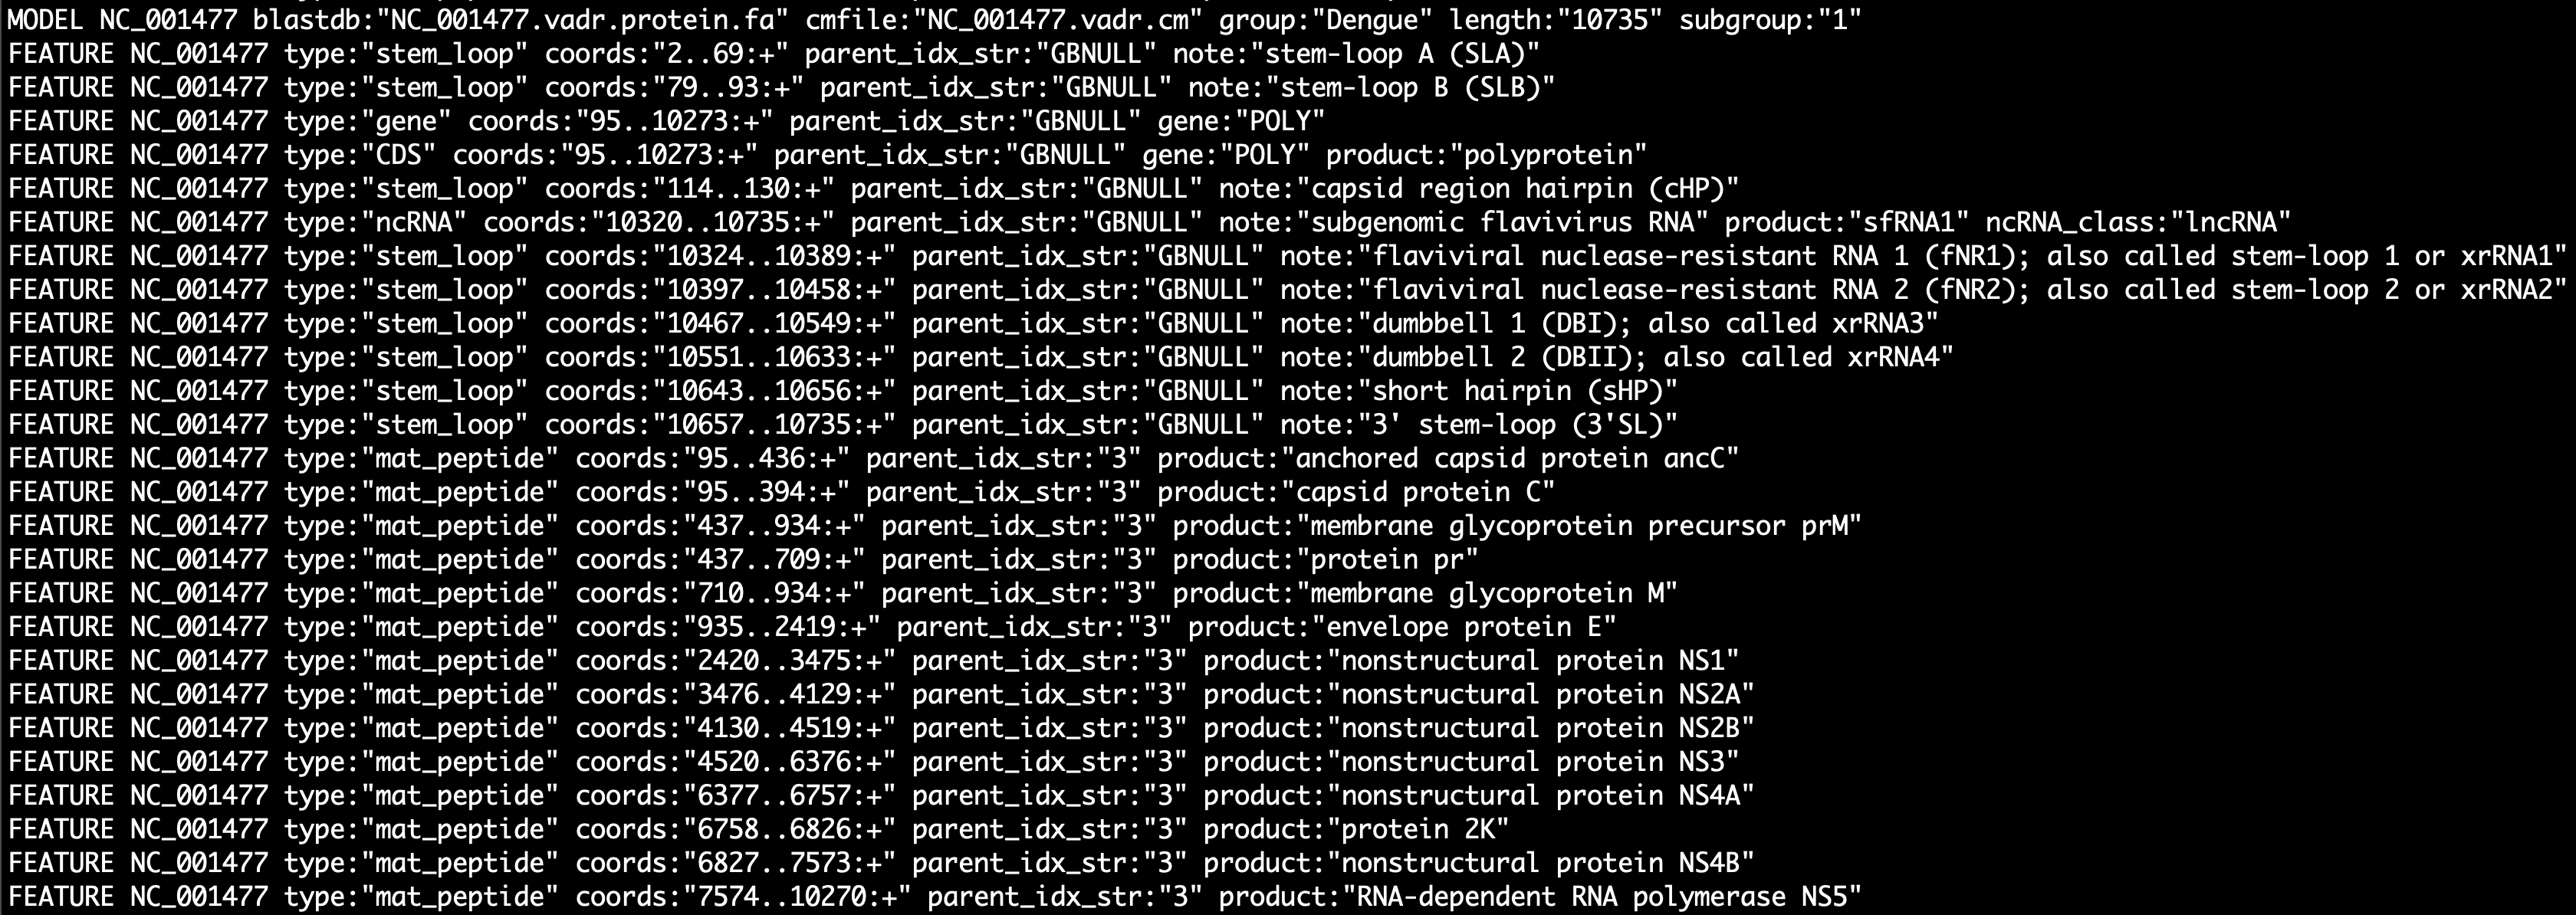
\includegraphics[width=10.5in]{figs/ss-001477-minfo}

\end{center}
\vfill
\end{slide}
%%%%%%%%%%%%%%%%%%%%%%%%%%%%%%%%%%%%%%%%%%%%%%%%%%%%%%%%%%%%%%%%%%%%%%
\begin{slide}
\begin{center}

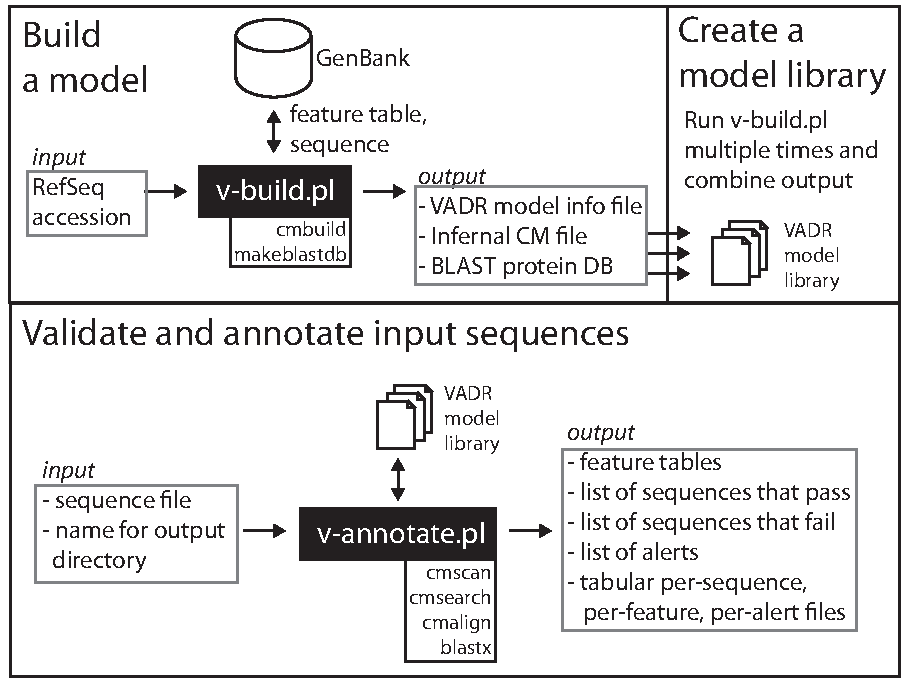
\includegraphics[width=8in]{figs/vadr}

\end{center}
\vfill
\end{slide}
%%%%%%%%%%%%%%%%%%%%%%%%%%%%%%%%%%%%%%%%%%%%%%%%%%%%%%%%%%%%%%%%%%%%%%
\begin{slide}
\begin{center}
\textbf{\texttt{v-annotate.pl} annotates each sequence using its
  best-matching model}

\small
\begin{description}
\item[Classification]: Each sequence is compared against all models 
  to determine its best-matching model to determine score only (no
  hit boundaries)

\item[Coverage determination]: Each sequence is compared against
  its best matching model again to obtain hit boundaries

\item[Alignment]: Each sequence is aligned to its best-matching
  model (globally with respect to sequence, locally with respect to
  the model) and feature annotation is mapped from model to sequence

\item[Protein validation]: Predicted CDS features in each sequence are
  compared against proteins from best-matching model using BLASTX
\end{description}

\emph{Different types of alerts are identified and reported at each stage}

\end{center}

\vfill
\end{slide}
%%%%%%%%%%%%%%%%%%%%%%%%%%%%%%%%%%%%%%%%%%%%%%%%%%%%%%%%%%%%%%%%%%%%%%
\begin{slide}
\begin{center}

\begin{description}
\item[Classification]: Each sequence is compared against all models 
  to determine its best-matching model to determine score only (no
  hit boundaries)
\end{description}

\begin{itemize} 
\item First 3 stages (only) of the HMMER3 pipeline are used to
  determine score quickly using a ``profile'' HMM of each model
  (single RefSeq).
\end{itemize}

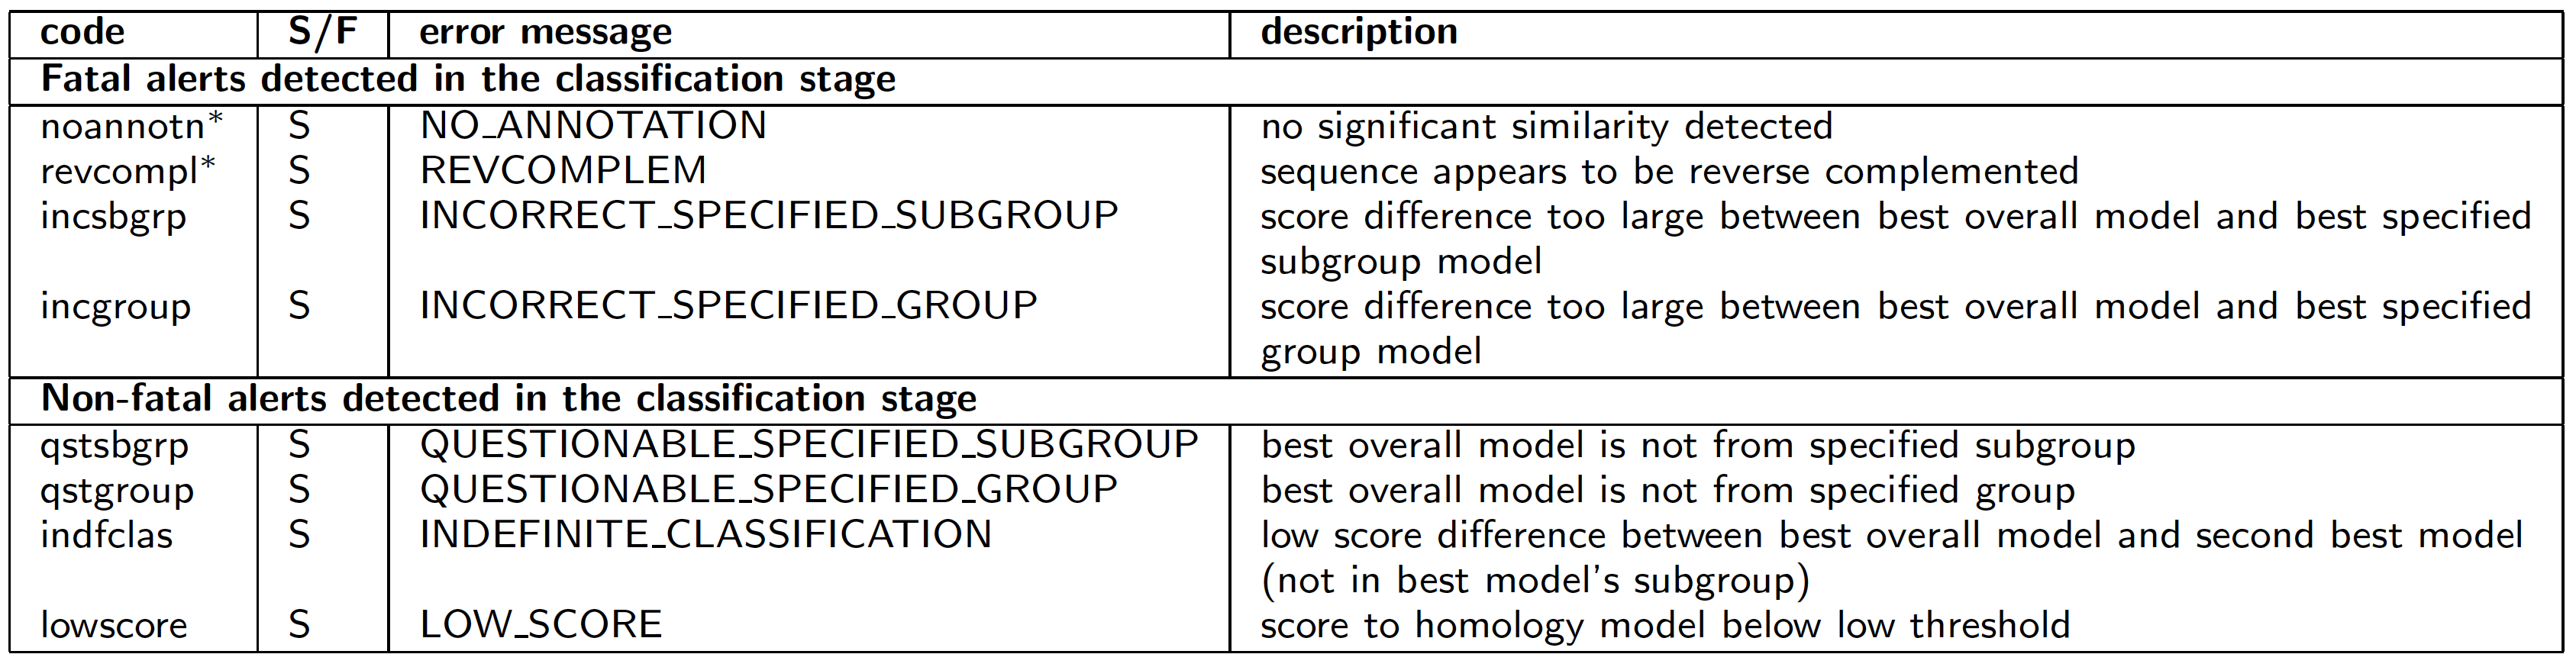
\includegraphics[width=10in]{figs/ss-class-alert-list}

\end{center}
\vfill
\end{slide}
%%%%%%%%%%%%%%%%%%%%%%%%%%%%%%%%%%%%%%%%%%%%%%%%%%%%%%%%%%%%%%%%%%%%%%
\begin{slide}
\begin{center}

\begin{description}
\item[Coverage determination]: Each sequence is compared against
  its best matching model again to obtain hit boundaries
\end{description}

\begin{itemize} 
\item Full HMMER3 pipeline is used using best-matching model to
  determine hit boundaries. Allows additional alert types to
  be detected.
\end{itemize}

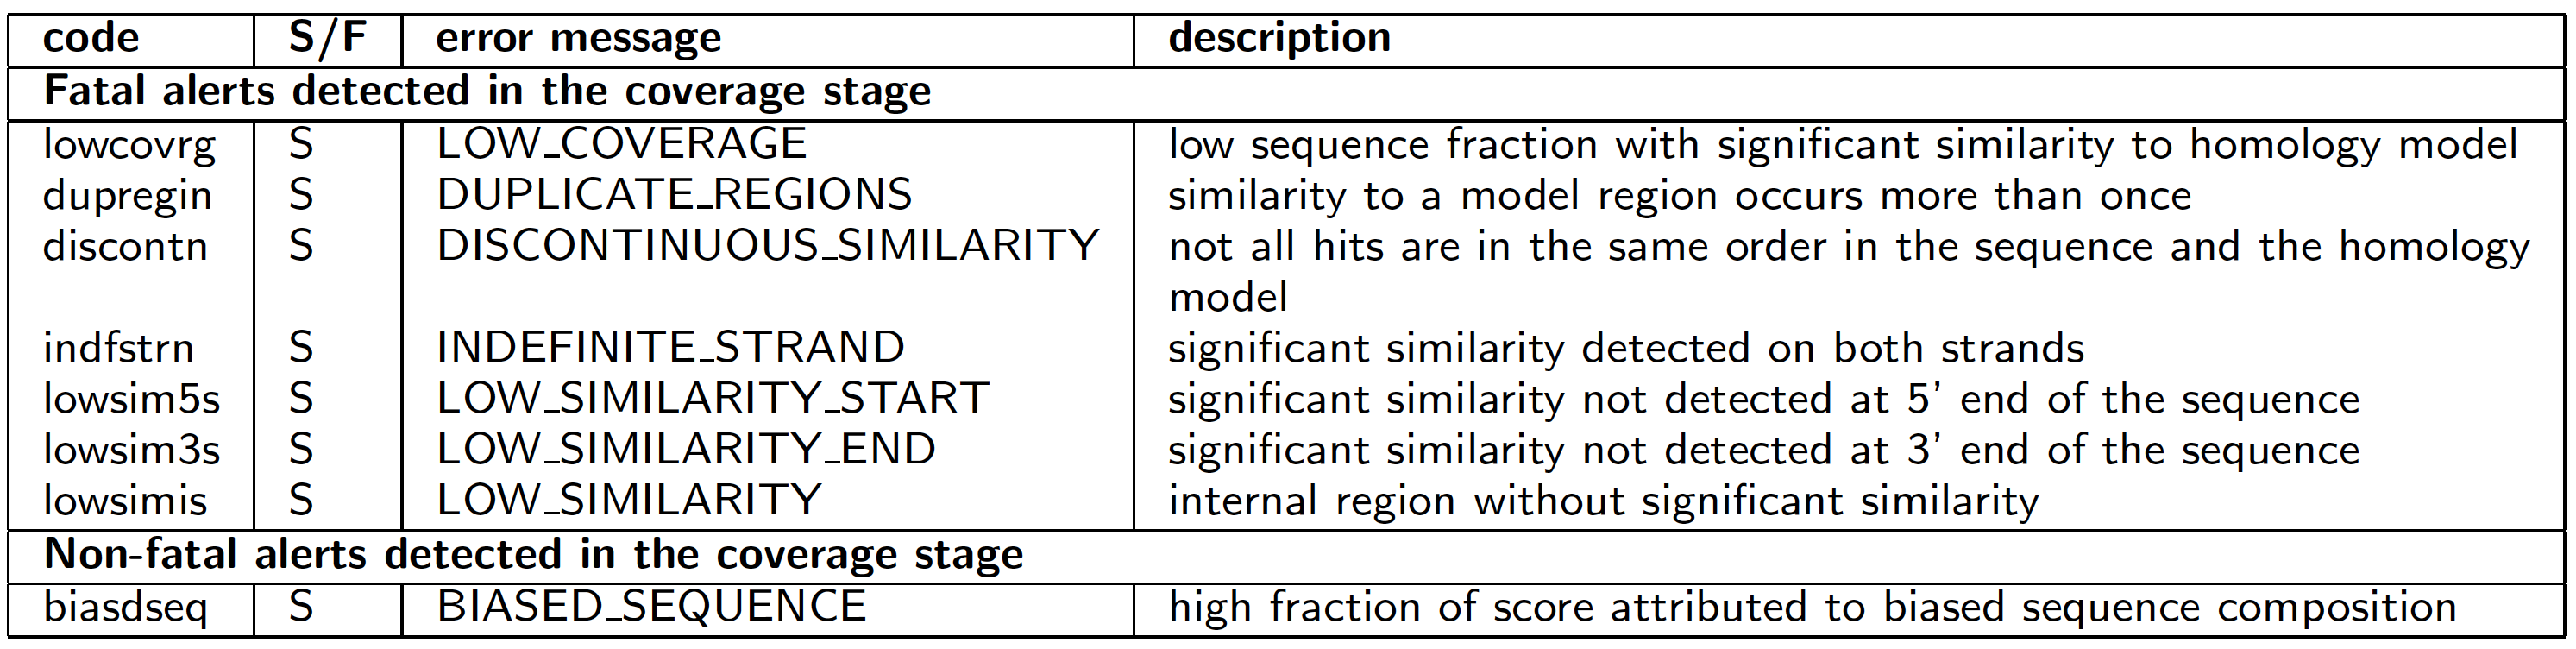
\includegraphics[width=10in]{figs/ss-coverage-alert-list}

\end{center}
\vfill
\end{slide}
%%%%%%%%%%%%%%%%%%%%%%%%%%%%%%%%%%%%%%%%%%%%%%%%%%%%%%%%%%%%%%%%%%%%%%
\begin{slide}
\begin{center}

\begin{description}
\item[Alignment]: Each sequence is aligned to its best-matching
  model (globally with respect to sequence, locally with respect to
  the model) and feature annotation is mapped from model to sequence
\end{description}

\begin{itemize} 
\item CM instead of HMMER3 HMM alignment is used to improve accuracy
  at at endpoints and allow structure information (when available). 
  Output includes posterior probabilities of aligned nucleotides.
\end{itemize}

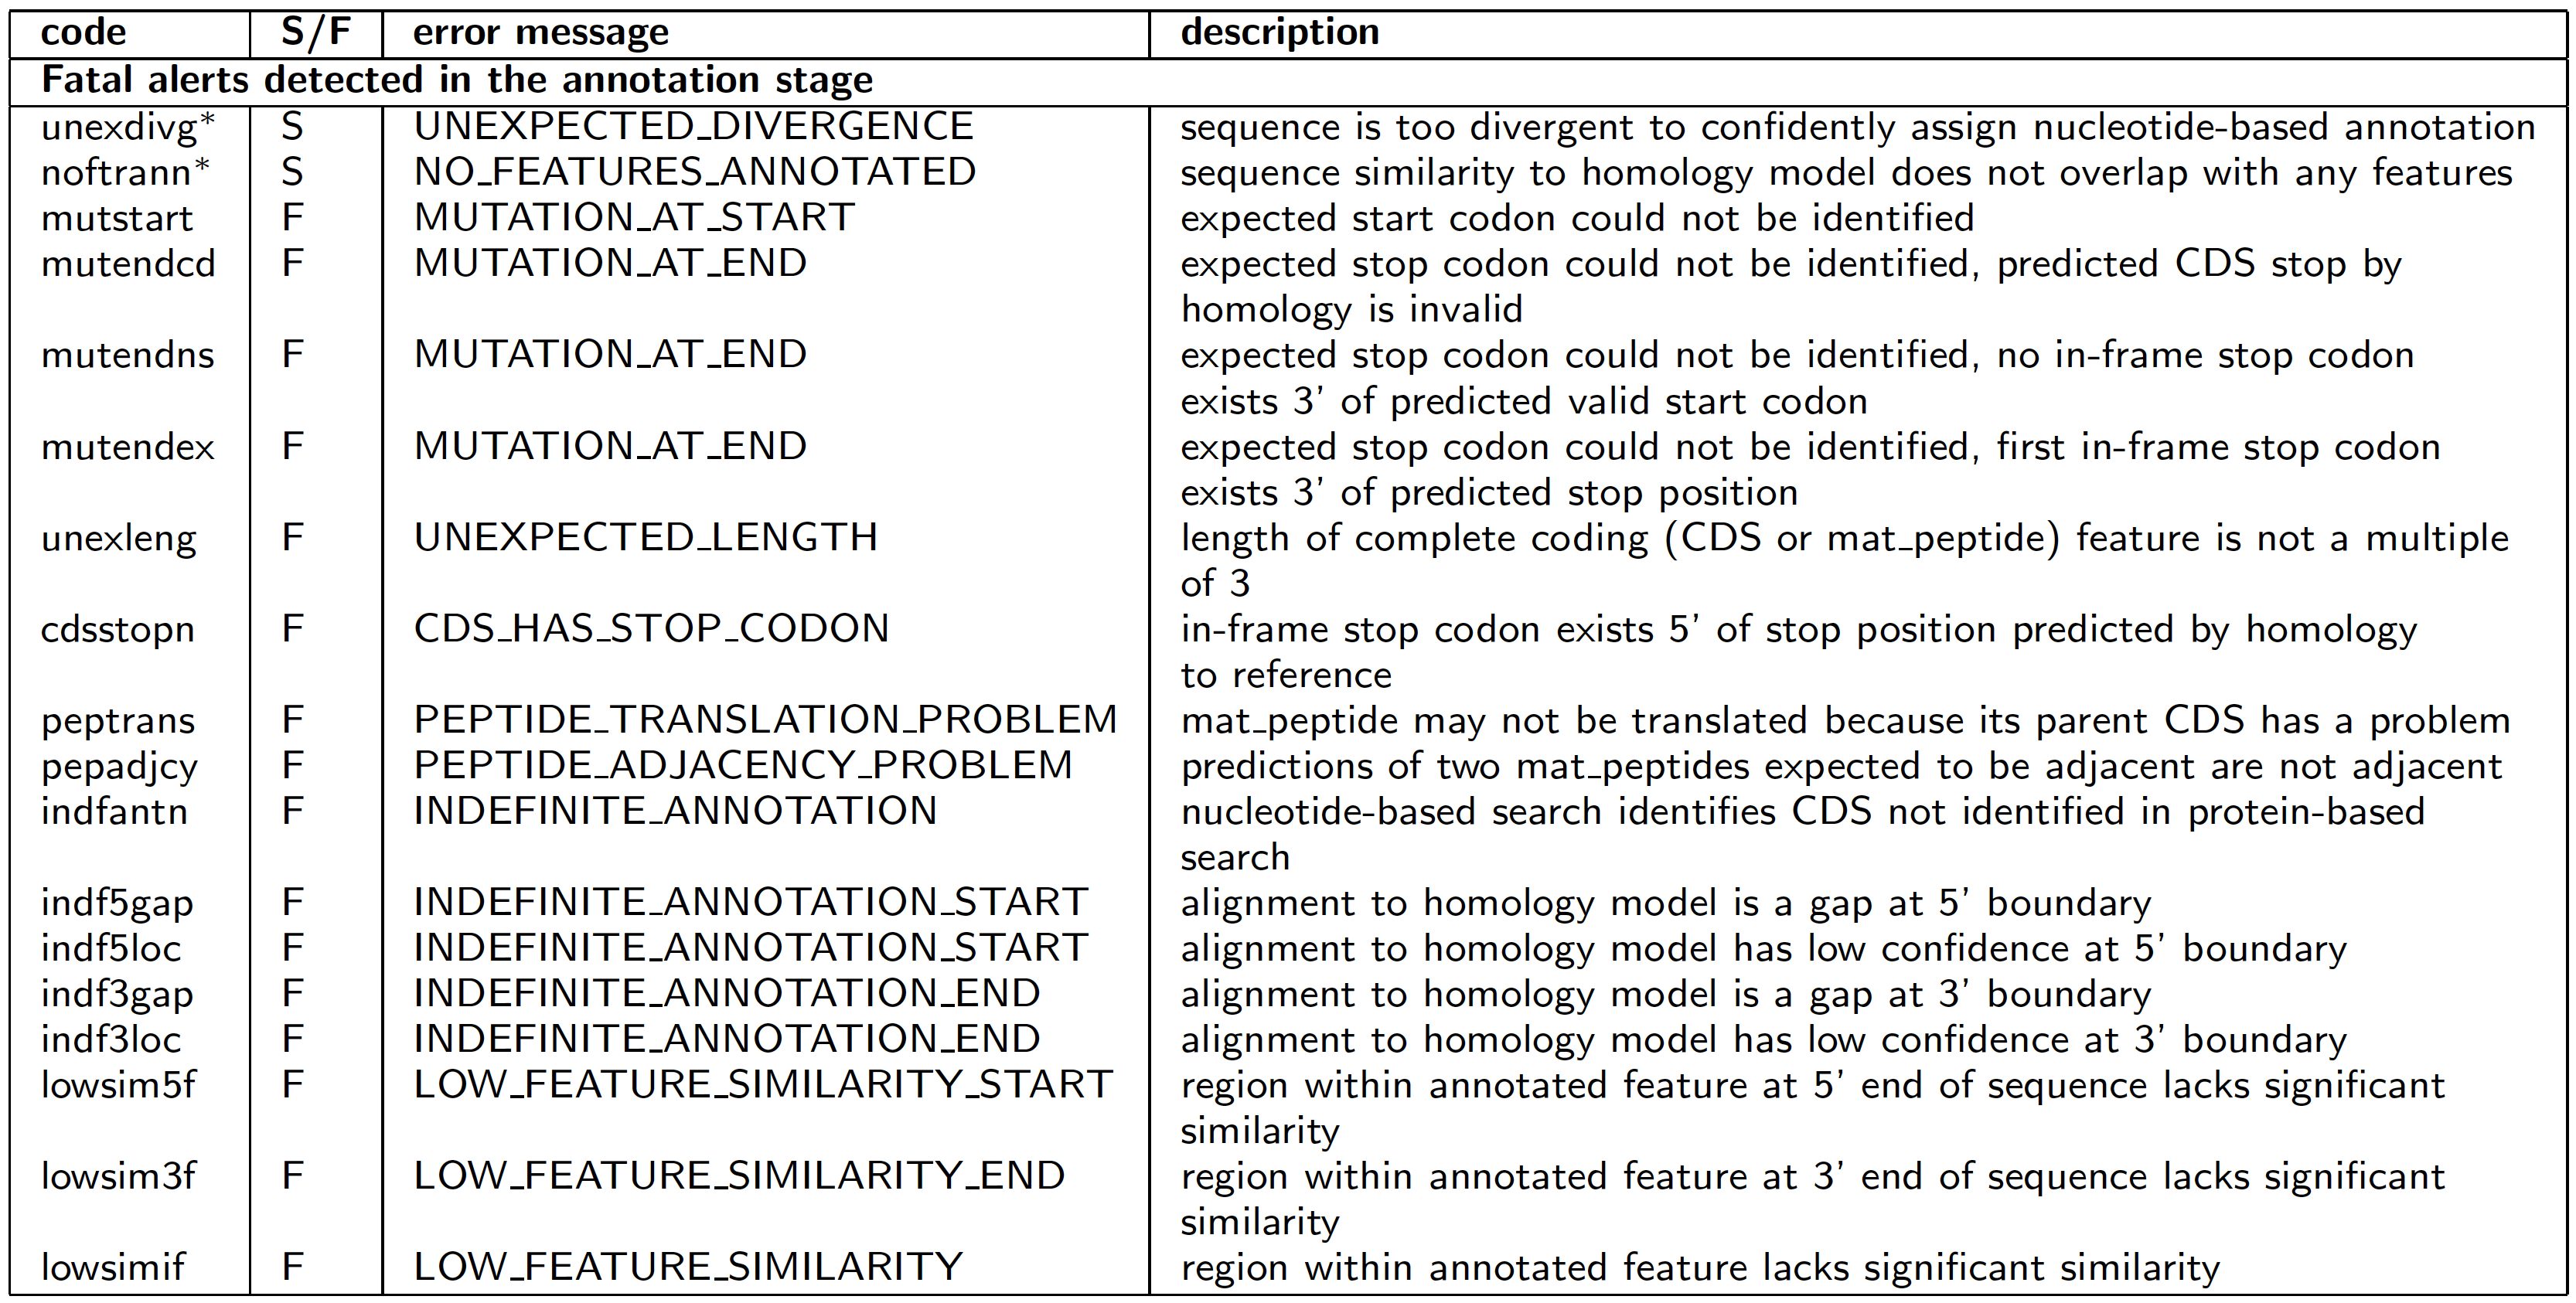
\includegraphics[width=10in]{figs/ss-alignment-alert-list}

\end{center}
\vfill
\end{slide}
%%%%%%%%%%%%%%%%%%%%%%%%%%%%%%%%%%%%%%%%%%%%%%%%%%%%%%%%%%%%%%%%%%%%%%
\begin{slide}
\begin{center}

\begin{description}
\item[Protein validation]: Predicted CDS features in each sequence are
  compared against proteins from best-matching model using BLASTX
\end{description}

\begin{itemize} 
\item Because other stages are nucleotide-based, frameshift mutations
  are not detected until this stage. Also maximum lengths for indels
  are enforced. 
\end{itemize}

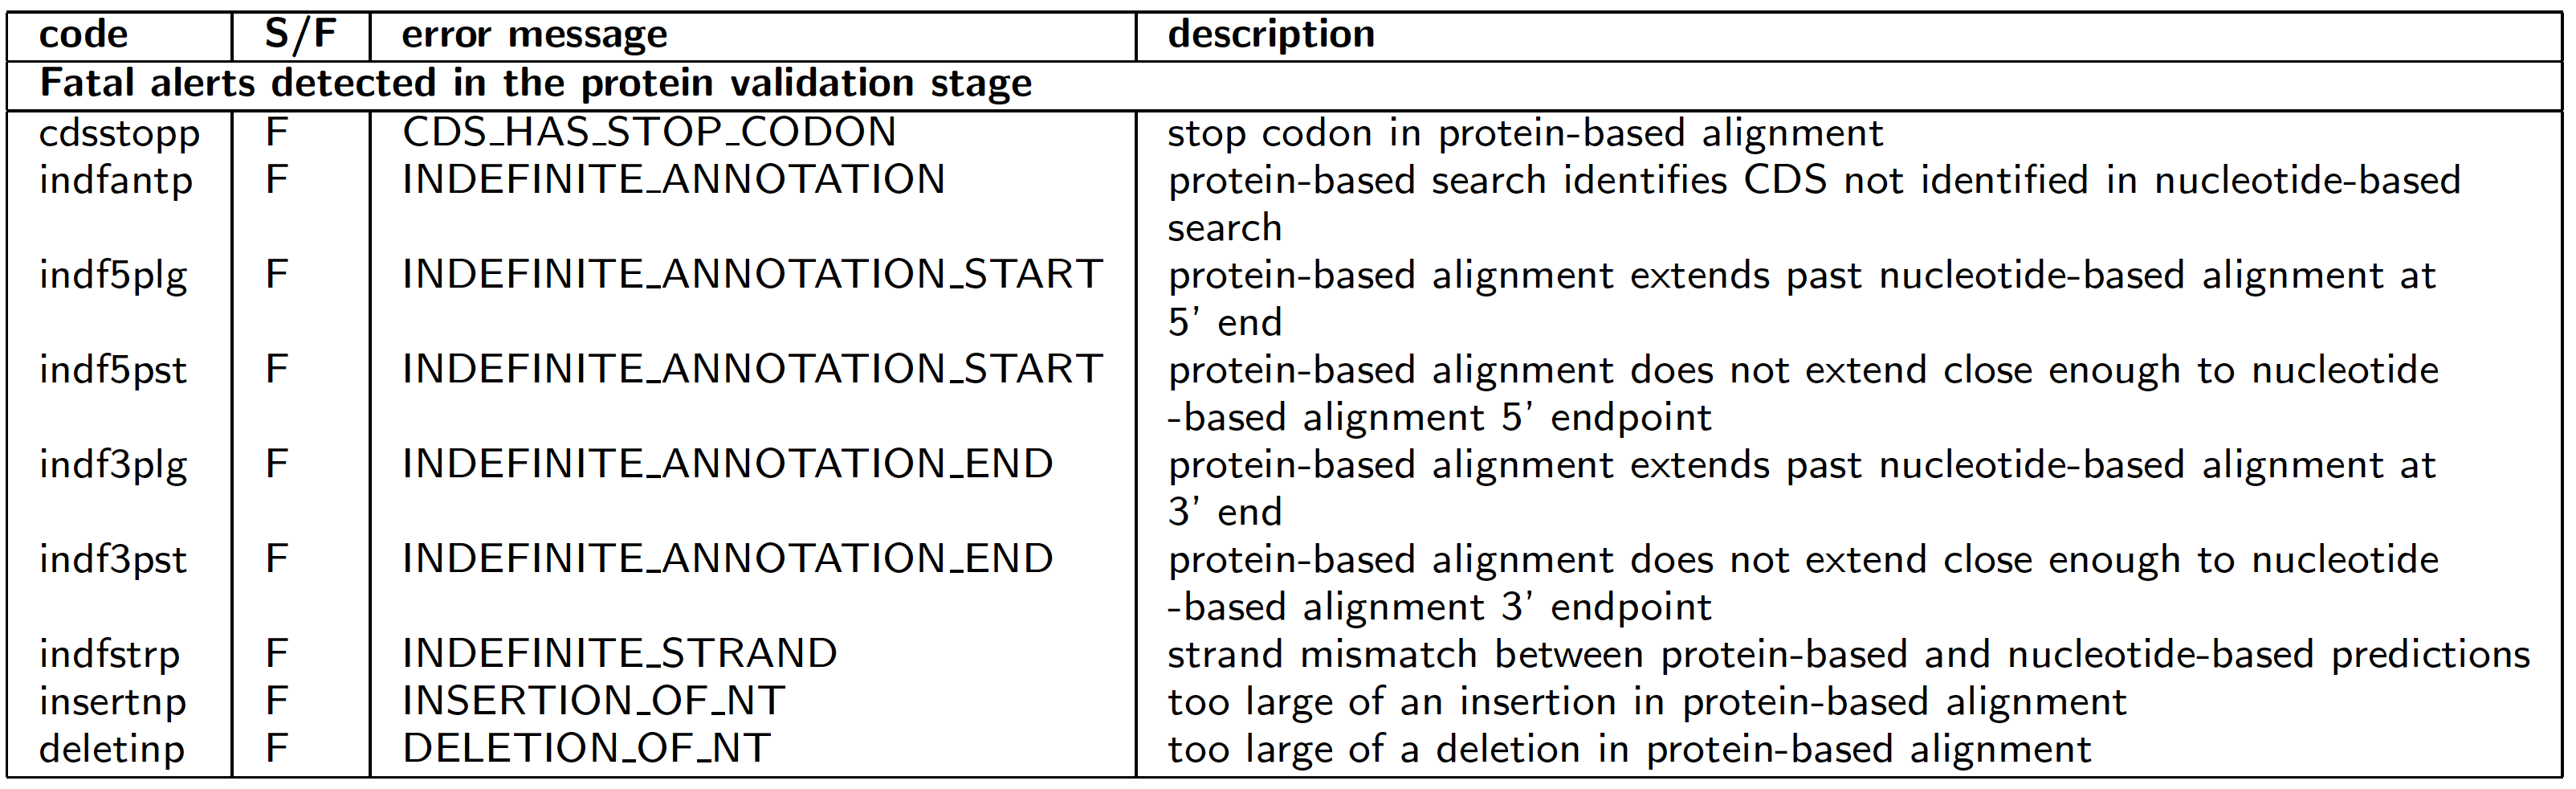
\includegraphics[width=10in]{figs/ss-protein-alert-list}

\end{center}
\vfill
\end{slide}
%%%%%%%%%%%%%%%%%%%%%%%%%%%%%%%%%%%%%%%%%%%%%%%%%%%%%%%%%%%%%%%%%%%%%%
%%%%%%%%%%%%%%%%%%%%%%%%%%%%%%%%%%%%%%%%%%%%%%%%%%%%%%%%%%%%%%%%%%%%%%%
\begin{slide}
\begin{center}
\textbf{VADR results on all Norovirus and Dengue sequences}

\scriptsize
\begin{tabular}{l|r|r|r|r|r}
                        &         & length       &         &         & fraction \\
 dataset                & \# seqs & range        & \# pass & \# fail & pass \\ \hline
Norovirus complete (NC) & 1384    & 7380..7839   & 1157    & 227     & 0.836 \\
Dengue complete (DC)    & 4580    & 10372..16254 & 4171    & 409     & 0.911 \\
& & & & & \\
Norovirus partial (NP)  & 32190   & 50..7376     & 29488   & 2702    & 0.916 \\
Dengue partial  (DP)    & 20973   & 50..10370    & 17276   & 3697    & 0.824 \\
\end{tabular}

\end{center}
\vfill
\end{slide}
%%%%%%%%%%%%%%%%%%%%%%%%%%%%%%%%%%%%%%%%%%%%%%%%%%%%%%%%%%%%%%%%%%%%%%
\begin{slide}
\begin{center}
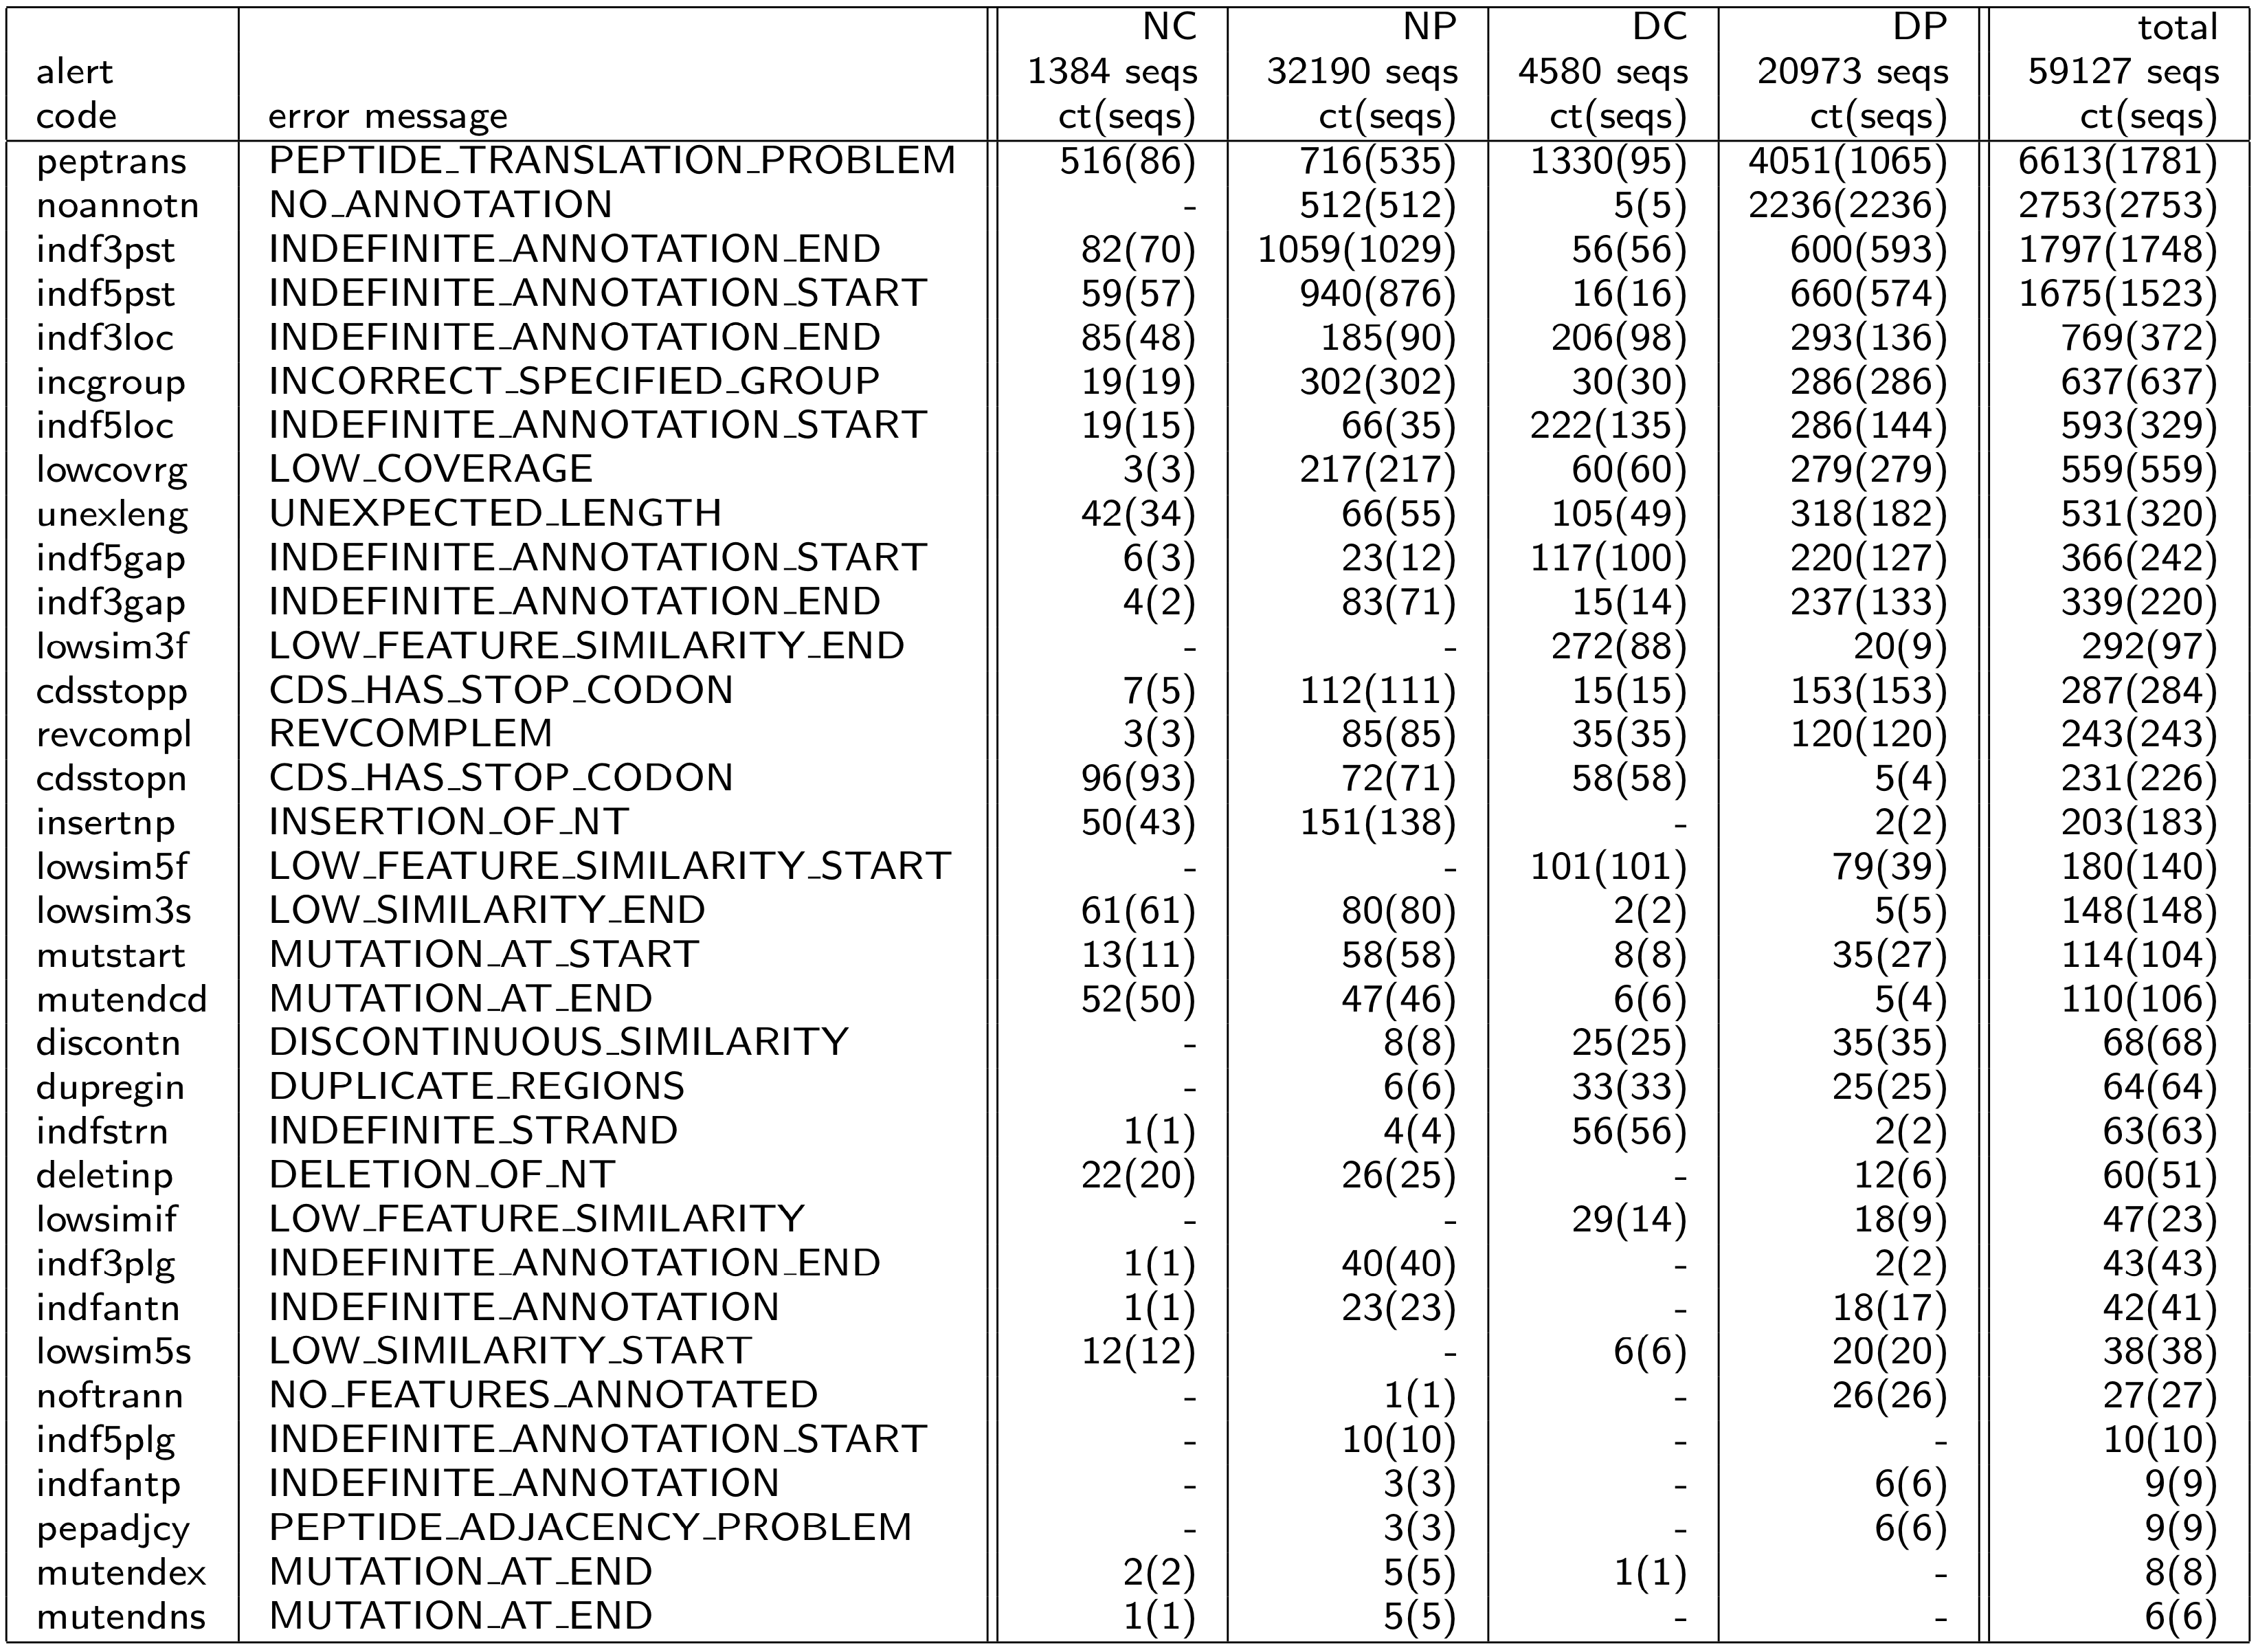
\includegraphics[width=10.5in]{figs/ss-alert-counts}
\end{center}

\vfill
\end{slide}
%%%%%%%%%%%%%%%%%%%%%%%%%%%%%%%%%%%%%%%%%%%%%%%%%%%%%%%%%%%%%%%%%%%%%%
\begin{slide}
\begin{center}

\includegraphics[width=10.5in]{figs/ss-vapid-title}
\end{center}

\small
\begin{itemize}
\item large reference database of nearly all complete genomes in
  GenBank
\item annotates each sequence based on best-match in reference
  database using blastn
\item designed for complete genomes
\item identifies early and absent stop codons and frameshift indels
\item simplifies submission by adding metadata expected by GenBank
\end{itemize}

\vfill
\end{slide}
%%%%%%%%%%%%%%%%%%%%%%%%%%%%%%%%%%%%%%%%%%%%%%%%%%%%%%%%%%%%%%%%%%%%%%
\begin{slide}
\begin{center}

\includegraphics[width=10.5in]{figs/ss-vigor-title}
\end{center}

\small
\begin{itemize}
\item determines most appropriate database (e.g. Norovirus)
  and annotates based on comparison of all proteins and mature
  peptides in that database
\item no Dengue database
\item identifies early and absent stop codons and frameshift indels
\end{itemize}

\vfill
\end{slide}
%%%%%%%%%%%%%%%%%%%%%%%%%%%%%%%%%%%%%%%%%%%%%%%%%%%%%%%%%%%%%%%%%%%%%%
\begin{slide}
\begin{center}
\textbf{Summary of VAPiD, VIGOR and VADR on 200 randomly chosen seqs}

\begin{tabular}{|l|r|r|r|}
\hline
         & VADR       & VAPiD     & VIGOR      \\
 dataset & pass/fail  & pass/fail & pass/fail  \\ \hline
       NC &  167/33 &  161/39 &   198/2 \\ 
       DC &  189/11 &   196/4 &       - \\ 
       NP &   191/9 &       - &   195/5 \\ 
       DP &  163/37 &       - &       - \\ 
\hline 
\end{tabular}
\end{center}

\vfill
\end{slide}
%%%%%%%%%%%%%%%%%%%%%%%%%%%%%%%%%%%%%%%%%%%%%%%%%%%%%%%%%%%%%%%%%%%%%%
\begin{slide}
\begin{center}
\textbf{Comparison of VAPiD and VADR}

\begin{tabular}{|l|r|r|r|r|}
\hline
          & Both       & Both       & VADR-pass  & VADR-fail  \\
 dataset  & pass       & fail       & VAPiD-fail & VAPiD-pass \\ \hline
       NC &        137 &          9 &         30 &     24 \\ 
       DC &        188 &          3 &          1 &      8 \\ 
\hline 
\end{tabular}

\end{center}

\vfill
\end{slide}
%%%%%%%%%%%%%%%%%%%%%%%%%%%%%%%%%%%%%%%%%%%%%%%%%%%%%%%%%%%%%%%%%%%%%%
\begin{slide}
\begin{center}
\textbf{Comparison of VAPiD and VADR}

\begin{tabular}{|l|r|r|r|r|}
\hline
          & Both       & Both       & VADR-pass  & VADR-fail  \\
 dataset  & pass       & fail       & VAPiD-fail & VAPiD-pass \\ \hline
       NC &        137 &          9 &         30 &     24 \\ 
       DC &        188 &          3 &          1 &      8 \\ 
\hline 
\end{tabular}

\small
\begin{itemize}
\item 12 that fail both:
  \begin{itemize}
  \item 9 have an internal stop (SEQ FEAT.InternalStop) or another
    CDS translation problem (SEQ FEAT.CdsTransFail)
  \item one has a start codon problem (SEQ FEAT.StartCodon)
  \item one is reverse complemented
  \item one fails because no reference is found
  \end{itemize}
\item 31 that fail only VAPiD are:
  \begin{itemize}
  \item either 5’ truncated in the first CDS, 3’ truncated in the
    final CDS, or both (at least one of SEQ FEAT.NoStop or SEQ FEAT.CdTransFail)
  \item 
    otherwise valid according to the VADR and VIGOR results
  \end{itemize}
\item \textcolor{red}{Conclusion: VADR finds all problems that VAPiD finds that should
  be caught.}
\end{itemize}
\end{center}

\vfill
\end{slide}
%%%%%%%%%%%%%%%%%%%%%%%%%%%%%%%%%%%%%%%%%%%%%%%%%%%%%%%%%%%%%%%%%%%%%%
\begin{slide}
\begin{center}
\textbf{Comparison of VIGOR and VADR}

\begin{tabular}{|l|r|r|r|r|}
\hline
         & Both       & Both       & VADR-pass  & VADR-fail  \\
 dataset & pass       & fail       & VIGOR-fail & VIGOR-pass \\ \hline
       NC &    167 &      2 &      0 &     31 \\ 
       NP &    191 &      5 &      0 &      4 \\ 
\hline 
\end{tabular}

\end{center}

\vfill
\end{slide}
%%%%%%%%%%%%%%%%%%%%%%%%%%%%%%%%%%%%%%%%%%%%%%%%%%%%%%%%%%%%%%%%%%%%%%
\begin{slide}
\begin{center}
\textbf{Comparison of VIGOR and VADR}

\begin{tabular}{|l|r|r|r|r|}
\hline
         & Both       & Both       & VADR-pass  & VADR-fail  \\
 dataset & pass       & fail       & VIGOR-fail & VIGOR-pass \\ \hline
      NC &        167 &          2 &          0 &     31 \\ 
      NP &        191 &          5 &          0 &      4 \\ 
\hline 
\end{tabular}

\small
\begin{itemize}
\item 7 that fail both:
  \begin{itemize}
  \item 3 have premature stops
  \item 2 are reverse complemented
  \item one has a frameshift 
  \item one fails because no similar reference is found
  \end{itemize}
\item \textcolor{red}{Conclusion: VADR finds all problems that VAPiD finds that should
  be caught.}
\end{itemize}
\end{center}

\vfill
\end{slide}

%%%%%%%%%%%%%%%%%%%%%%%%%%%%%%%%%%%%%%%%%%%%%%%%%%%%%%%%%%%%%%%%%%%%%%
\begin{slide}
\begin{center}
\textbf{35 sequences in NC, DC, and NP fail only VADR}

\small
\begin{itemize}
\item \textcolor{red}{These all have issues indexers want to manually review:}
\begin{itemize}
\item 16 sequences with early stops compared to closest RefSeqs %(\emph{cdsstopn})
\item 12 sequences for which BLASTX alignment does not extend close
  enough to alignment-based prediction %(\emph{indf5pst}, \emph{indf3pst})
\item 10 sequences with low similarity to RefSeq at 5' or 3' end of
  sequence or a feature %(lowsim5f, lowsim3f, or lowsim3s alerts)
\item 7 sequences where 5' or 3' boundary is a gap or not aligned with
  sufficient confidence (high enough posterior probability)
  %(indf5loc, indf5gap, or indf3loc alerts)
\item 5 sequences that are expected to be Norovirus but are really Sapovirus
  %(incgroup alerts)
\item 5 sequences with too large of an insertion/deletion in the
  BLASTX alignment %(insertnp or deletinp alerts)
\item 1 sequence not recognized by any of the \emph{Caliciviridae} or
  \emph{Flaviviridae} models (a Salivirus from \emph{Picornaviridae}
  family) %(noannotn alert)
\end{itemize}
\end{itemize}
\end{center}

\vfill
\end{slide}
%%%%%%%%%%%%%%%%%%%%%%%%%%%%%%%%%%%%%%%%%%%%%%%%%%%%%%%%%%%%%%%%%%%%%%
\begin{slide}
\begin{center}
\textbf{VADR documentation?}
\end{center}

\vfill
\end{slide}
%%%%%%%%%%%%%%%%%%%%%%%%%%%%%%%%%%%%%%%%%%%%%%%%%%%%%%%%%%%%%%%%%%%%%%
\begin{slide}
\begin{center}
\textbf{Future directions}
\end{center}

\begin{itemize}
\item alignment-based models 
\item profile-based protein validation replace BLASTX
\item extend to more genes, including ribosomal RNAs and possible ITS
  sequences 
\end{itemize}

\vfill
\end{slide}
%%%%%%%%%%%%%%%%%%%%%%%%%%%%%%%%%%%%%%%%%%%%%%%%%%%%%%%%%%%%%%%%%%%%%%%%
\begin{slide}
\begin{center}
\textbf{Limitations}
\end{center}

\begin{itemize}
\item works in nucleotide space
\item RefSeq or alignment must be 'representative'
  \begin{itemize}
    \item any sequence that is not conserved is challenging
    \item introns in random positions are problematic
    \item different gene order is problematic
  \end{itemize}
\item current length limit of model is about 20Kb (CM alignment memory
  requirements)
\item slow
\end{itemize}

\vfill
\end{slide}
%%%%%%%%%%%%%%%%%%%%%%%%%%%%%%%%%%%%%%%%%%%%%%%%%%%%%%%%%%%%%%%%%%%%%%
%%%%%%%%%%%%%%%%%%%%%%%%%%%%%%%%%%%%%%%%%%%%%%%%%%%%%%%%%%%%%%%%%%%%%%%%%
\begin{slide}

\large
\begin{center}
\large{\textbf{Acknowledgements}} \\

\normalsize
\vspace{0.75in}

\small
\begin{tabular}{l|l|l}
%                  & \\ \hline
%                  & \\
\textbf{NCBI - viral annotation} & \textbf{NCBI - leadership} &  \textbf{HMMER} \\
Alejandro Sch\"{a}ffer           & David Landsman             & Sean Eddy \\
Rodney Brister                   & Jim Ostell                 & Travis Wheeler \\
Ilene Mizrachi                   & David Lipman               & \\
Eneida Hatcher                   & & \\
Linda Yankie                     & & \\
Alex Kotliarov                   & & \\
Susan Schafer                    & & \\
Lara Shonkwiler                  & & \\
Sophia Hu                        & & \\
\end{tabular}


\includegraphics[width=2.5in]{figs/NIH_NLM_ABRV_2C_4-white}

\includegraphics[width=2.5in]{figs/ncbi-logo}

\end{center}

\vfill
\end{slide}


\end{document}
%%%%%%%%%%%%%%%%%%%%%%%%%%%%%%%%%%%%%%%%%%%%%%%%%%%%%%%%%%%%%%%%%%%%%%
%%%%%%%%%%%%%%%%%%%%%%%%%%%%%%%%%%%%%%%%%%%%%%%%%%%%%%%%%%%%%%%%%%%%%%
%%%%%%%%%%%%%%%%%%%%%%%%%%%%%%%%%%%%%%%%%%%%%%%%%%%%%%%%%%%%%%%%%%%%%%
%%%%%%%%%%%%%%%%%%%%%%%%%%%%%%%%%%%%%%%%%%%%%%%%%%%%%%%%%%%%%%%%%%%%%%
%%%%%%%%%%%%%%%%%%%%%%%%%%%%%%%%%%%%%%%%%%%%%%%%%%%%%%%%%%%%%%%%%%%%%%
%%%%%%%%%%%%%%%%%%%%%%%%%%%%%%%%%%%%%%%%%%%%%%%%%%%%%%%%%%%%%%%%%%%%%%
\begin{slide}
\begin{center}
\textbf{Sequence submissions are handled by expert NCBI indexers}
\end{center}

\small
\begin{itemize}
\item Indexers check submissions for quality
\item Many submissions are of \emph{marker genes}, used to
  characterize environments (microbiome, soil), which are
  automatically analyzed by BLAST or specialized tools.
%\item Submissions with zero errors automatically enter database
%  (``foosh'')
%\item Submissions with errors can be corrected by submitter or are manually reviewed by an indexer
\end{itemize}

\medskip

\begin{center}
\begin{tabular}{l||r|r||r||l}
                                 &    2018  & total     &         &           \\
 marker gene/                    &  GenBank & GenBank   &  TLS\footnote{TLS: Targeted Locus Study, currently only 16S submissions with $>=$ 2500 seqs}      & analysis  \\
 sequence type                   &  \# seqs & \# seqs   & \# seqs & tool \\ \hline
& & & \\                    
%\textcolor{red}{16S rRNA}        & \textcolor{red}{333,121}  & \textcolor{red}{8,015,297} & \textcolor{red}{18,262,402} & \textcolor{red}{BLAST}\footnote{TLS submissions now processed with Ribosensor} \\
%16S rRNA                        & 333,121  & 8,015,297 & 18,262,402 & BLAST$^{*}$ \\
16S rRNA                        & 333,121  & 8,015,297 & 18,262,402 & BLAST \\
& & & \\                    
 23S rRNA                        & 74,287  &   275,014  & 2,140      & BLAST \\
& & & \\
 ITS1                            & 27,279  &   359,380  & 13,294     & BLAST \\
& & & \\                    
 ITS2                            & 24,144  &   184,515  &      0     & BLAST \\
& & & \\                    
 ITS1+ITS2                       & 26,734  &   445,721  & 25,725     & BLAST \\
& & & \\                    
 Influenza A                     & 74,868  &   665,464  &      0     & FLAN \\
\end{tabular}
\end{center}
\vfill
\tiny \flushleft{$\dagger$ TLS: Targeted Locus Study, currently only 16S submissions with $>=$ 2500 seqs, handled by Anji Johnston}
%\tiny \flushleft{$\ddagger$ TLS submissions now processed with ribosensor}
\end{slide}
